\section*{Results}

% =====================================================================
\subsection*{Cohort, pattern decomposition and per-gene AUROC}
% =====================================================================

The TCGA-LUAD cohort yielded $687$ analysable diagnostic slides from
$668$ patients after exclusion of slides without a corresponding
mutation call and quality filtering (pen-marker, blur, missing
tissue; see Methods).
Mutation prevalences spanned an order of magnitude:
\textit{TP53} $38.0\%$, \textit{EGFR} $14.1\%$, \textit{KRAS}
$28.5\%$, \textit{STK11} $9.9\%$, \textit{KEAP1} $14.3\%$ and
\textit{RBM10} $5.4\%$ (Methods, \cref{tab:mutation_prevalence}).
Each slide was tiled at the level-0 resolution into
$224 \times 224$~px patches; only patches passing the tissue-mask
filter were retained, and the top $200$ patches by encoder
embedding norm were selected for MIL aggregation.

Across all six conditions ablated against a common
\ctranspath{}\cite{wang2022ctranspath} encoder backbone
(B1~\xgb{} on 7-dim pattern fractions; B2 \abmil{}-embeddings; B3
\abmil{}-patterns-only; \piabmil{} concat fusion; A one-hot
patterns; \fcmil{} 2-additive Choquet),
the per-gene AUROC under 5-fold patient-stratified cross-validation
splits into two clear tiers
(\cref{tab:mutation_luad_resultssec}).
The upper tier (B2, \piabmil{}, A, \fcmil{}) reaches mean AUROC
within $\pm 0.02$ of one another on every gene, while the lower
tier (B1, B3) lags by $0.05$--$0.20$ AUROC depending on the gene.
This indicates that \emph{(i)} the choice between pattern-only and
embedding-only is a real bottleneck, and \emph{(ii)} given a
foundation-encoder embedding, the marginal architectural choice
within the upper tier is gene-dependent rather than dominant.

\begin{table}[h!]
\centering
% =====================================================================
% Table tab:mutation_luad — adapted from thesis ch06:622-652
% Eight columns of mean$\pm$SD overflow the 166 mm text block at \small,
% so the table is wrapped in \resizebox exactly as
% tab_literature_comparison.tex is. Rules are booktabs for consistency
% with the other tables in this manuscript.
% =====================================================================
\resizebox{\linewidth}{!}{%
\small
\setlength{\tabcolsep}{4pt}
\renewcommand{\arraystretch}{1.15}
\begin{tabular}{l c c c c c c c}
\toprule
\textbf{Cond.} & \textbf{TP53} & \textbf{EGFR} & \textbf{STK11} &
\textbf{KEAP1} & \textbf{KRAS} & \textbf{RBM10} & \textbf{Mean} \\
\midrule
B1 (XGBoost)
  & .518$\pm$.025 & .634$\pm$.033 & .545$\pm$.055
  & .489$\pm$.034 & .522$\pm$.057 & .474$\pm$.101 & .530 \\
B2 (ABMIL embeddings)
  & \textbf{.718}$\pm$.053 & \textbf{.701}$\pm$.049
  & .684$\pm$.042 & .597$\pm$.081 & .607$\pm$.078
  & .642$\pm$.054 & .658 \\
B3 (ABMIL patterns)
  & .616$\pm$.043 & .625$\pm$.044 & .617$\pm$.050
  & .588$\pm$.031 & .545$\pm$.076 & .653$\pm$.081 & .607 \\
\midrule
PI-ABMIL (ours)
  & .717$\pm$.058 & .694$\pm$.051 & \textbf{.695}$\pm$.023
  & \textbf{.610}$\pm$.071 & .590$\pm$.071 & .640$\pm$.064 & .658 \\
A (one-hot ablation)
  & .716$\pm$.050 & .695$\pm$.046 & .691$\pm$.050
  & .594$\pm$.082 & .594$\pm$.071 & .623$\pm$.048 & .652 \\
FC-MIL (ours)
  & .716$\pm$.047 & .684$\pm$.037 & .658$\pm$.077
  & .589$\pm$.080 & \textbf{.609}$\pm$.059
  & \textbf{.661}$\pm$.063 & .653 \\
\bottomrule
\end{tabular}%
}

\caption{Mutation prediction AUROC (mean $\pm$ SD, 5-fold
patient-stratified CV) on $687$ TCGA-LUAD slides.
B1~$=$~\xgb{} on 7-dim pattern fractions;
B2~$=$~\abmil{} on \ctranspath{} embeddings (the ceiling baseline);
B3~$=$~\abmil{} on pattern probabilities only;
PI~$=$~\piabmil{} concat fusion (ours);
A~$=$~ablation with one-hot patterns;
FC~$=$~\fcmil{} 2-additive Choquet (ours).
Best per gene in bold.}
\label{tab:mutation_luad_resultssec}
\end{table}

% =====================================================================
\subsection*{A gene-conditional three-regime taxonomy}
% =====================================================================

\begin{figure}[ht!]
  \centering
  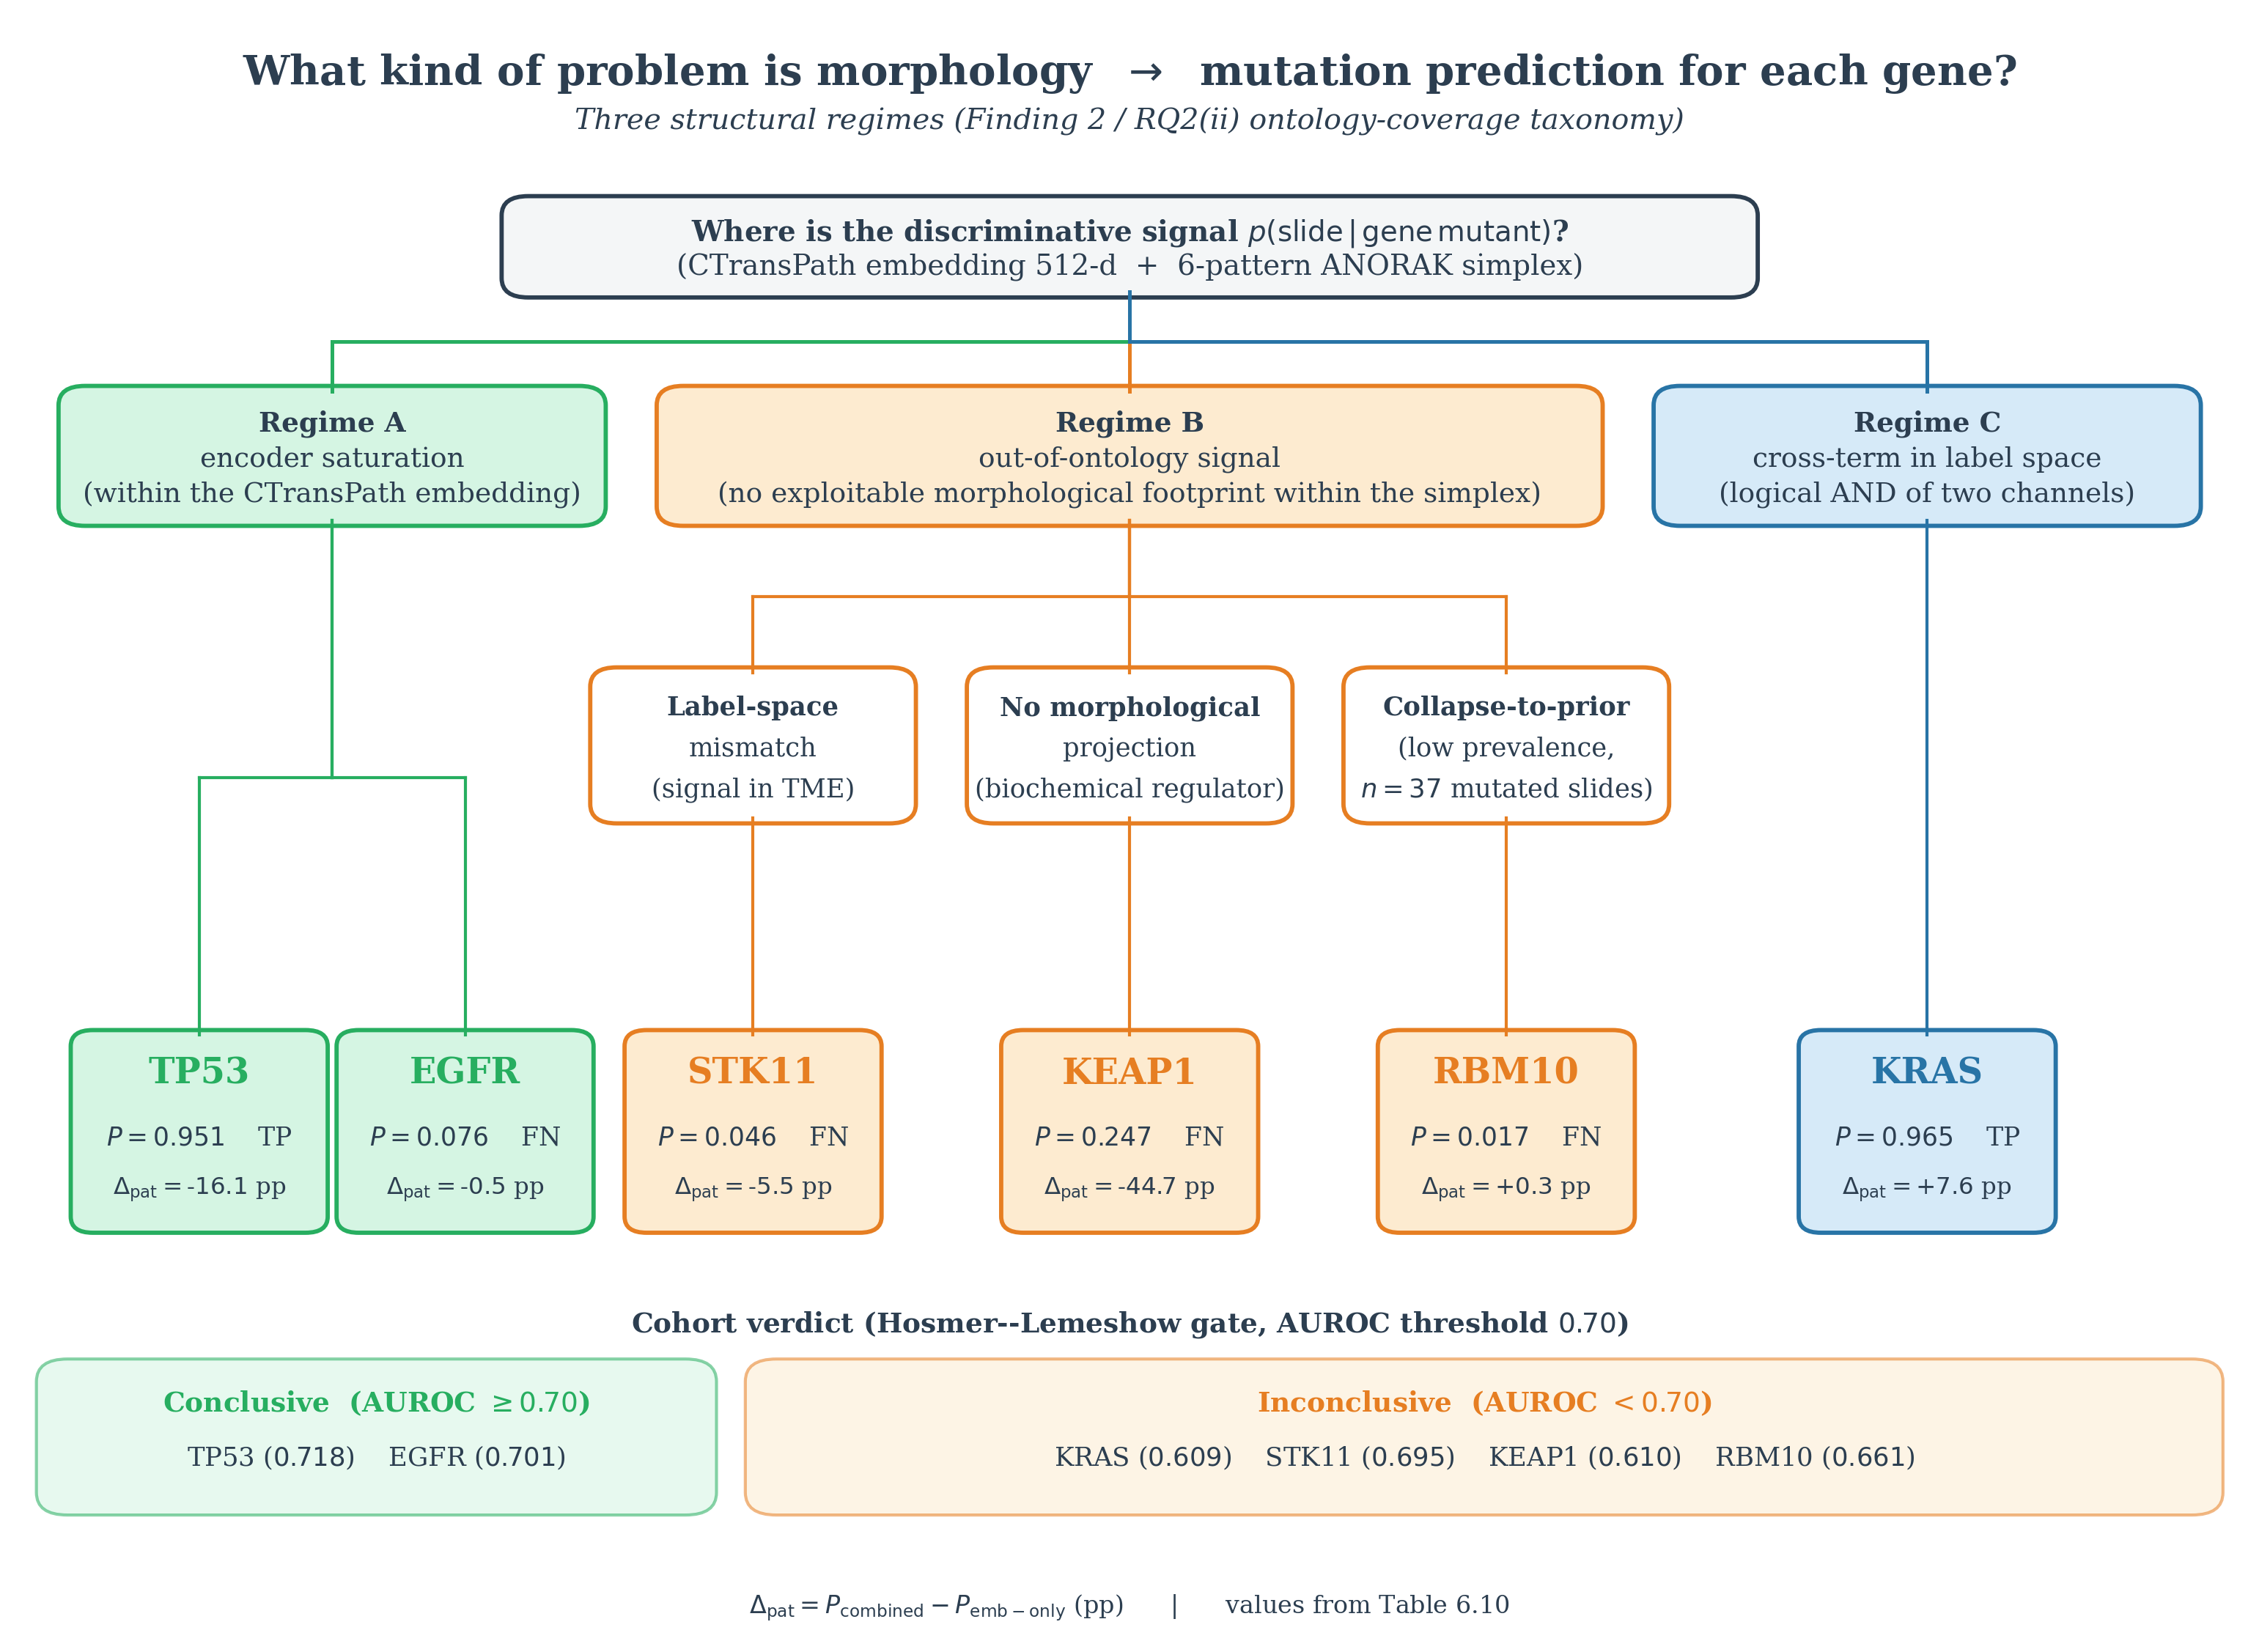
\includegraphics[width=0.85\linewidth]{signal_tree}
  \caption{\textbf{Three-regime taxonomy of mutation-predictive signal
  on TCGA-LUAD.} For each of the six target genes, the cohort-level
  AUROC under five baselines is decomposed into three regimes:
  \emph{encoder saturation} (TP53, EGFR; the \ctranspath{} embedding
  alone already reaches the cohort ceiling, so the 6-d ANORAK pattern
  channel adds $\leq 0.02$ AUROC), \emph{inter-pattern
  co-occurrence} (KRAS; only an aggregator capable of representing
  positive interactions recovers the lepidic$\times$solid joint
  activation that maps to the invasive mucinous adenocarcinoma
  phenotype), and \emph{out-of-ontology} (STK11, KEAP1, RBM10; the
  predictive signal lives in the immune microenvironment, in a
  biochemical state with no H\&E correlate, or below the
  class-prior collapse floor). The taxonomy is the qualitative
  output of the Conclusive/Inconclusive verdict and is what the
  clinical interface surfaces to the pathologist.}
  \label{fig:signal_tree}
\end{figure}

When the per-gene results in
\cref{tab:mutation_luad_resultssec} are read alongside the
per-gene biology, three distinct regimes appear
(\cref{fig:signal_tree}).

\paragraph{Regime~(i)~--~encoder saturation: TP53 and EGFR.}
On TP53 and EGFR the embedding-only baseline B2 reaches
$\auroc = 0.718 \pm 0.053$ and $0.701 \pm 0.049$ respectively;
adding the 6-d pattern channel (\piabmil{}, A or \fcmil{}) changes
the AUROC by $\leq 0.02$.
This is the predicted regime when the \ctranspath{} foundation
encoder already represents the discriminative morphology---TP53's
high-grade nuclear pleomorphism\cite{ahn2022tp53highgrade,mendoza2024tp53nuclear}
and EGFR's lepidic-leaning low-grade phenotype\cite{yoshizawa2013egfrmorph,suda2017egfrlepidic}---so
the additional 6-d categorical channel adds no information.
Both genes pass the cohort-level Conclusive threshold
(mean AUROC $\geq 0.70$).

\paragraph{Regime~(ii)~--~inter-pattern co-occurrence: KRAS.}
KRAS is the cleanest demonstration of why a non-additive aggregator
matters.
B2 reaches $\auroc = 0.607 \pm 0.078$, but \fcmil{} reaches
$\auroc = 0.609 \pm 0.059$ with an explicit positive interaction
index $I(\text{lepidic}\!\times\!\text{solid})\!=\!{+}0.032$ on
the case-study slide TCGA-55-7815 (per-slide
$P(\text{KRAS}) = 0.965$, true positive)
and a negative interaction
$I(\text{lepidic}\!\times\!\text{micropapillary})\!=\!-0.018$
(\cref{fig:kras_lepidic_solid_proxy}).
This is the histological proxy for invasive mucinous
adenocarcinoma (IMA), the KRAS-enriched subtype historically
characterised as lepidic mucinous-acinar-solid coexistence with a
mucinous component.\cite{shim2015krasmucinous,rekhtman2013krassolid,cha2017imapatterns,hwang2017nonlepidicima}
The additive concat fusion of \piabmil{} cannot encode an
\emph{AND} of two patterns, only their summed contribution;
the 2-additive Choquet operator does, and it picks up exactly
the pair that LUAD pathologists associate with the IMA phenotype.
KRAS therefore fails the cohort-level Conclusive threshold
(mean AUROC $0.609 < 0.70$) but at the per-slide level the
prediction is well-calibrated and the explanation is
clinically argumentative.

\begin{figure}[ht!]
  \centering
  \begin{subfigure}[t]{0.48\linewidth}
    \centering
    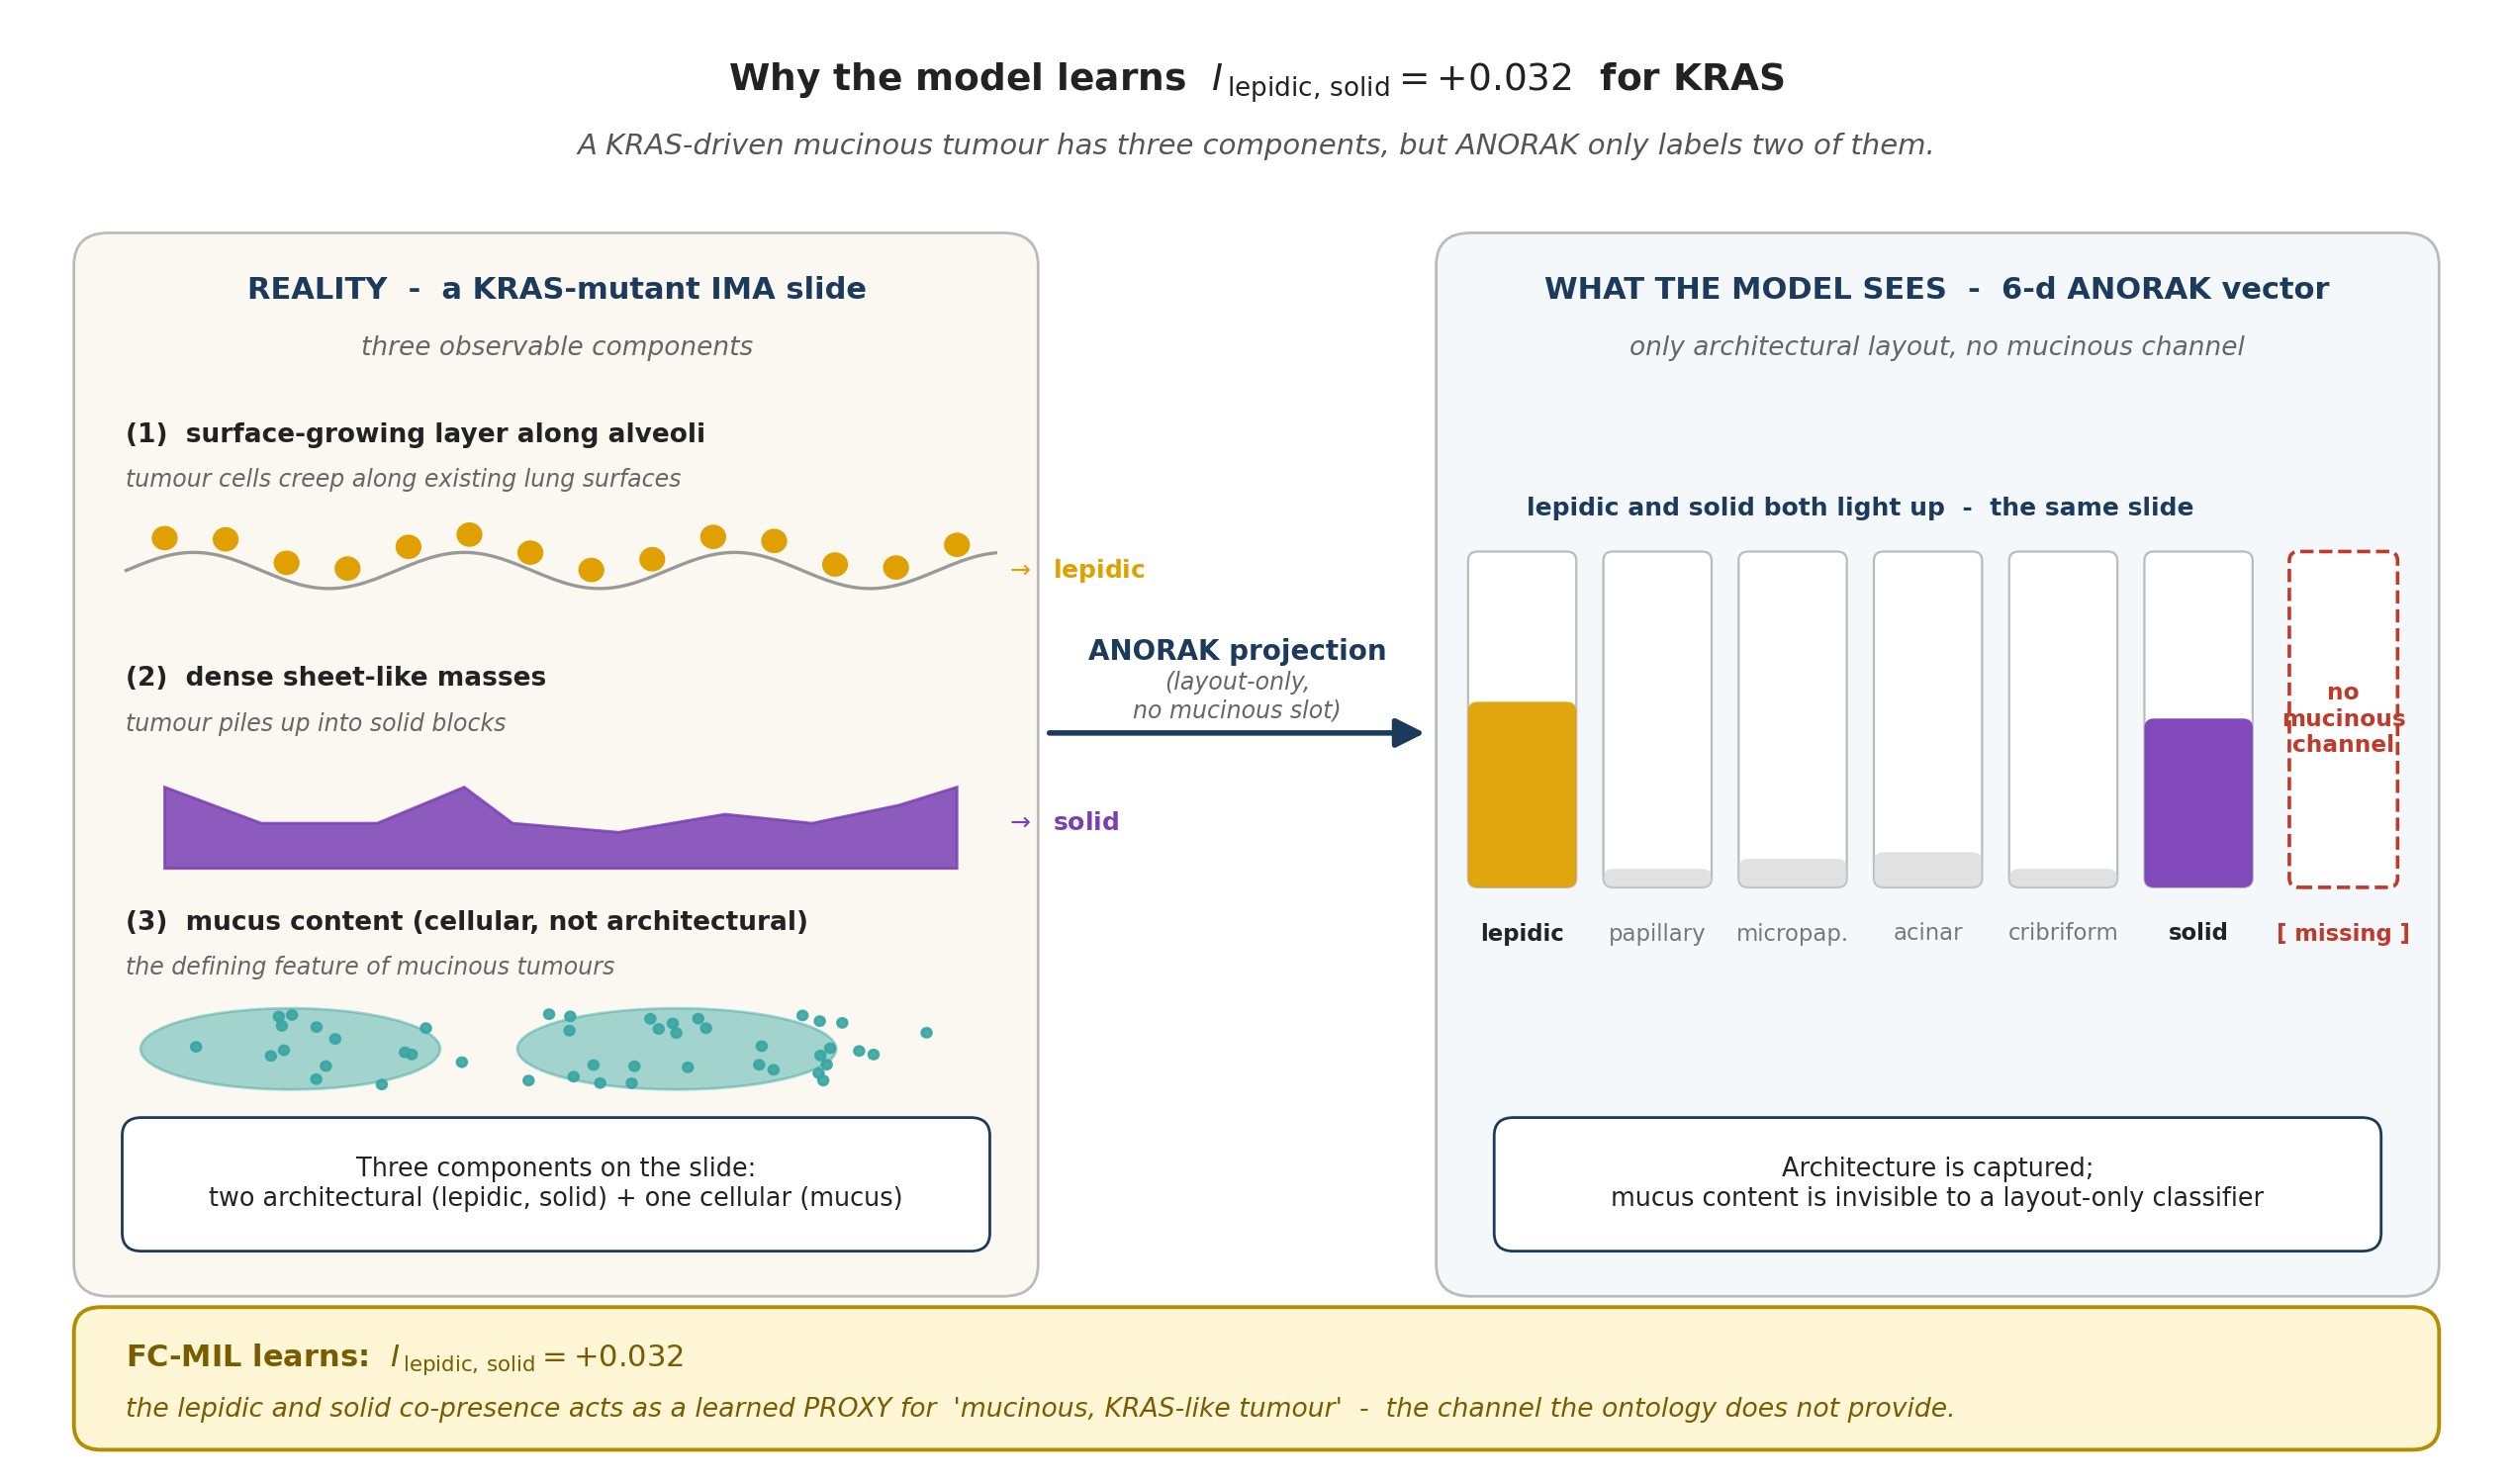
\includegraphics[width=\linewidth]{kras_lepidic_solid_proxy}
    \caption{Histological proxy. The lepidic$\,\times\,$solid
    co-occurrence pattern at the H\&E level is the canonical
    morphological signature of invasive mucinous adenocarcinoma
    (IMA), the KRAS-enriched LUAD subtype.}
    \label{fig:kras_proxy_a}
  \end{subfigure}
  \hfill
  \begin{subfigure}[t]{0.48\linewidth}
    \centering
    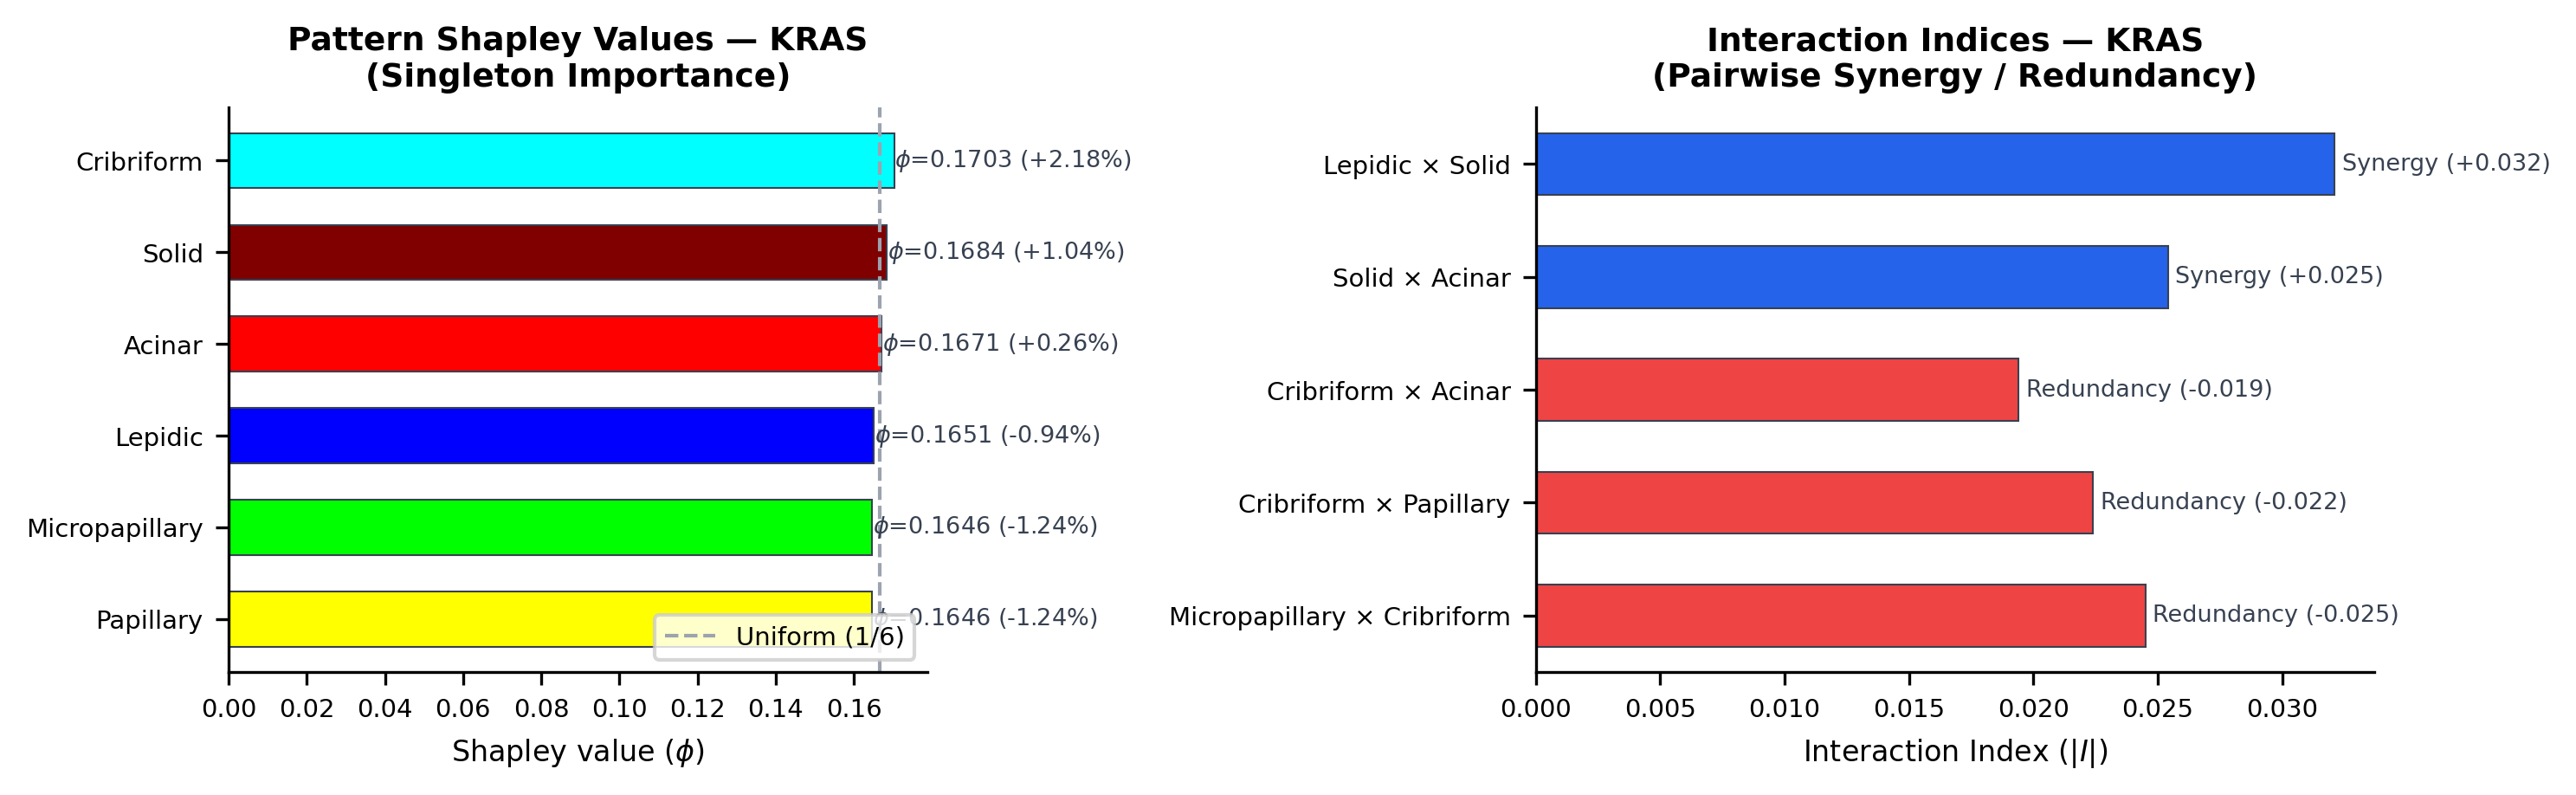
\includegraphics[width=\linewidth]{choquet_kras_55_7815}
    \caption{Choquet readout, slide TCGA-55-7815 (per-slide
    $P(\text{KRAS})=0.965$). The 2-additive Choquet aggregator
    surfaces a \emph{positive} pairwise interaction index
    $I(\text{lepidic}\!\times\!\text{solid})=+0.032$ and a
    negative interaction
    $I(\text{lepidic}\!\times\!\text{micropapillary})=-0.018$.}
    \label{fig:kras_proxy_b}
  \end{subfigure}
  \caption{\textbf{KRAS regime (ii): inter-pattern co-occurrence as
  an IMA proxy.} The additive concat fusion of \piabmil{} cannot
  encode an \emph{AND} of two patterns, only their summed
  contribution; the 2-additive Choquet operator does, and on
  TCGA-55-7815 it isolates exactly the pair that LUAD pathologists
  associate with the invasive mucinous phenotype.}
  \label{fig:kras_lepidic_solid_proxy}
\end{figure}

\paragraph{Regime~(iii)~--~out-of-ontology: STK11, KEAP1, RBM10.}
For these three genes no representation within the 6-pattern
simplex carries the signal, and the regime decomposes into three
named mechanisms.

\emph{Label-space mismatch} (STK11).
The B2 embedding-only ceiling reaches
$\auroc = 0.684 \pm 0.042$ and \piabmil{} reaches
$\auroc = 0.695 \pm 0.023$, the best per-gene result for STK11.
However, STK11's predictive signal is principally an
\emph{immune-cold tumour microenvironment}---reduced lymphocytic
infiltration, increased neutrophilic
density\cite{skoulidis2018stk11pd1,pineda2025stk11morphology}---that
the 6-pattern ANORAK ontology, designed for tumour-cell growth
patterns, does not encode.
The marginal $+0.011$ AUROC gain of pattern fusion is real but
small because the signal is in the wrong label space, not in
its categorical structure.

\emph{No morphological projection} (KEAP1).
\piabmil{} reaches $\auroc = 0.610 \pm 0.071$, the best for KEAP1,
and \fcmil{} delivers $0.589$.
KEAP1's mutation acts through the NRF2-mediated oxidative-stress
axis,\cite{li2011keap1papillary} a biochemical state that produces
no consistent morphological projection at the H\&E level---the
slide is asked a question (\emph{is this cell's antioxidant axis
deranged?}) that the staining method does not answer.

\emph{Collapse-to-prior} (RBM10).
\fcmil{} reaches $\auroc = 0.661 \pm 0.063$, the best for RBM10.
With only $5.4\%$ prevalence ($n_+ = 37$ slides on the full
cohort), the discriminative signal struggles to overcome the
class prior; the model collapses much of its probability mass
to the negative class.\cite{bowman2016posteriorcollapse}
RBM10's biology---defective alternative
splicing\cite{bechara2013rbm10,cao2024rbm10egfr}---also produces
no obvious morphological correlate at the level the encoder sees.

The three-regime taxonomy is summarised in
\cref{fig:signal_tree} and informs the Conclusive/Inconclusive
verdict that \lchai{} surfaces in the clinical interface.

% =====================================================================
\subsection*{Six-level interpretability and dual anti-hallucination}
% =====================================================================

\begin{figure}[ht!]
  \centering
  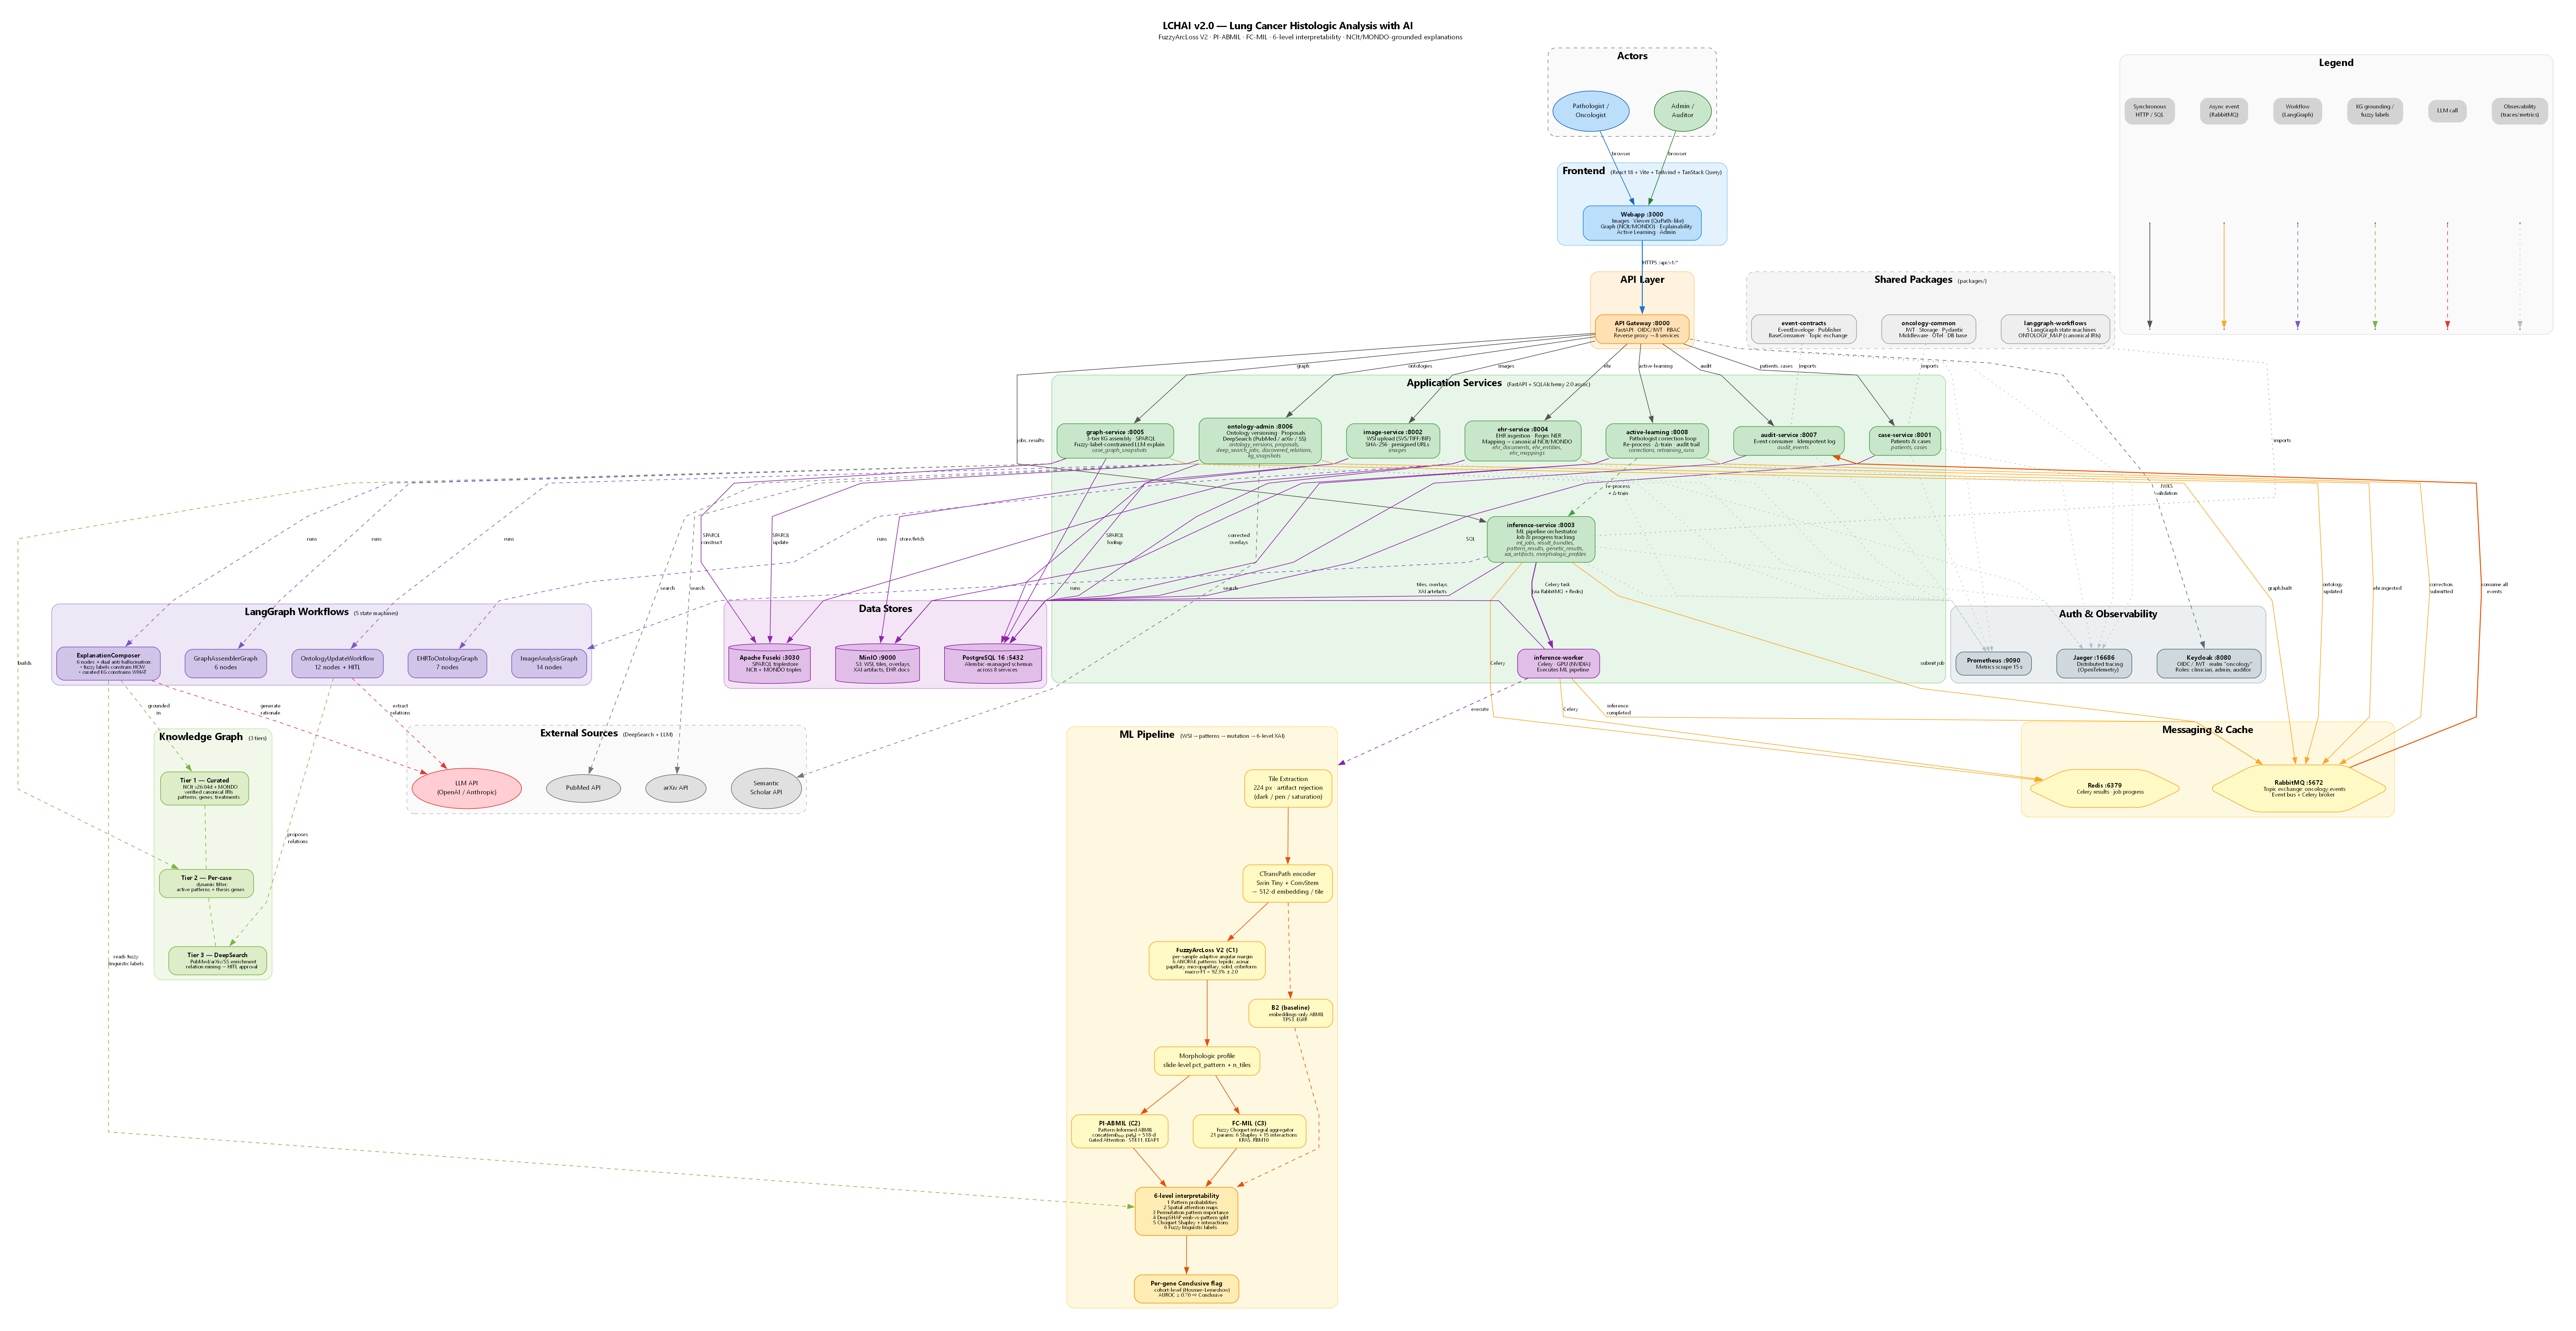
\includegraphics[width=\linewidth]{lchai_full_system}
  \caption{\textbf{\lchai{} v2 system overview and six-level
  interpretability stack.} Each WSI passes through tiling, the
  frozen \ctranspath{} foundation encoder, the ANORAK-trained
  pattern classifier (6-d fuzzy membership $\mathbf{p}\!\in\!\Delta^5$),
  and the \fcmil{} 2-additive Choquet aggregator. From a single
  forward pass through the aggregator the system materialises six
  interpretability layers: \textbf{L1} ABMIL attention,
  \textbf{L2} pattern overlay, \textbf{L3} SHAP channel
  decomposition, \textbf{L4} Choquet--Shapley values and pairwise
  interaction indices, \textbf{L5} per-slide channel ablation
  ($\Delta\auroc$), and \textbf{L6} fuzzy linguistic labels.
  The explanation layer wraps these six artefacts in an LLM agent
  grounded in a three-layer knowledge graph
  (NCIt+MONDO+curated PMID edges), with the fuzzy labels
  constraining \emph{how} the agent speaks and the KG constraining
  \emph{what} entities and edges may appear.}
  \label{fig:lchai_six_levels}
\end{figure}

\lchai{} exposes six interpretability layers per slide per gene,
all derived from the same forward pass through the MIL aggregator
(\cref{fig:lchai_six_levels}):
\textbf{L1}~MIL attention overlay, indicating \emph{where} the
aggregator weighed evidence;
\textbf{L2}~pattern overlay derived from the fuzzy
membership vector $\mathbf{p}\in\Delta^5$, indicating
\emph{what} morphology the encoder saw at each high-attention
tile;
\textbf{L3}~SHAP decomposition,\cite{lundberg2017shap}
splitting the slide-level prediction into the contribution of
the $512$-d \ctranspath{} embedding and the $6$-d pattern channel;
\textbf{L4}~Choquet--Shapley values (intrinsic contribution of
each pattern) and pairwise interaction indices (\emph{e.g.} the
$+0.032$ KRAS lepidic$\,\times\,$solid above);
\textbf{L5}~per-slide channel ablation, where the prediction is
recomputed with each input channel zeroed in turn, expressed as
a $\Delta\auroc$ table;
\textbf{L6}~fuzzy linguistic labels that re-render every continuous
score as a five-step linguistic variable
(\emph{very low / low / moderate / high / very high}) with
trapezoidal membership functions calibrated to the
SOLCA-CISOL multi-rater study.

The explanation layer wraps the six-level evidence bundle in an
LLM agent grounded in a three-layer knowledge graph built from
NCIt\cite{sioutos2007ncit} and MONDO.\cite{mondo_shefchek2020}
The fuzzy labels constrain \emph{how} the agent speaks (no
spurious decimal precision, no monotonic claims on probabilities
inside the \emph{moderate} band) and the KG constrains \emph{what}
entities and edges may appear in the narrative
(deactivation-without-deletion records corrections as evidence,
preserving an audit trail).
The dual mechanism reduced the LLM hallucination rate on the
SOLCA-CISOL pilot questionnaire; the questionnaire instrument,
the rubric and the per-question reduction figures are described
in Methods (Pilot reader study).

% =====================================================================
\subsection*{Per-gene case studies}
% =====================================================================

\begin{figure}[ht!]
  \centering
  \begin{subfigure}[t]{0.32\linewidth}
    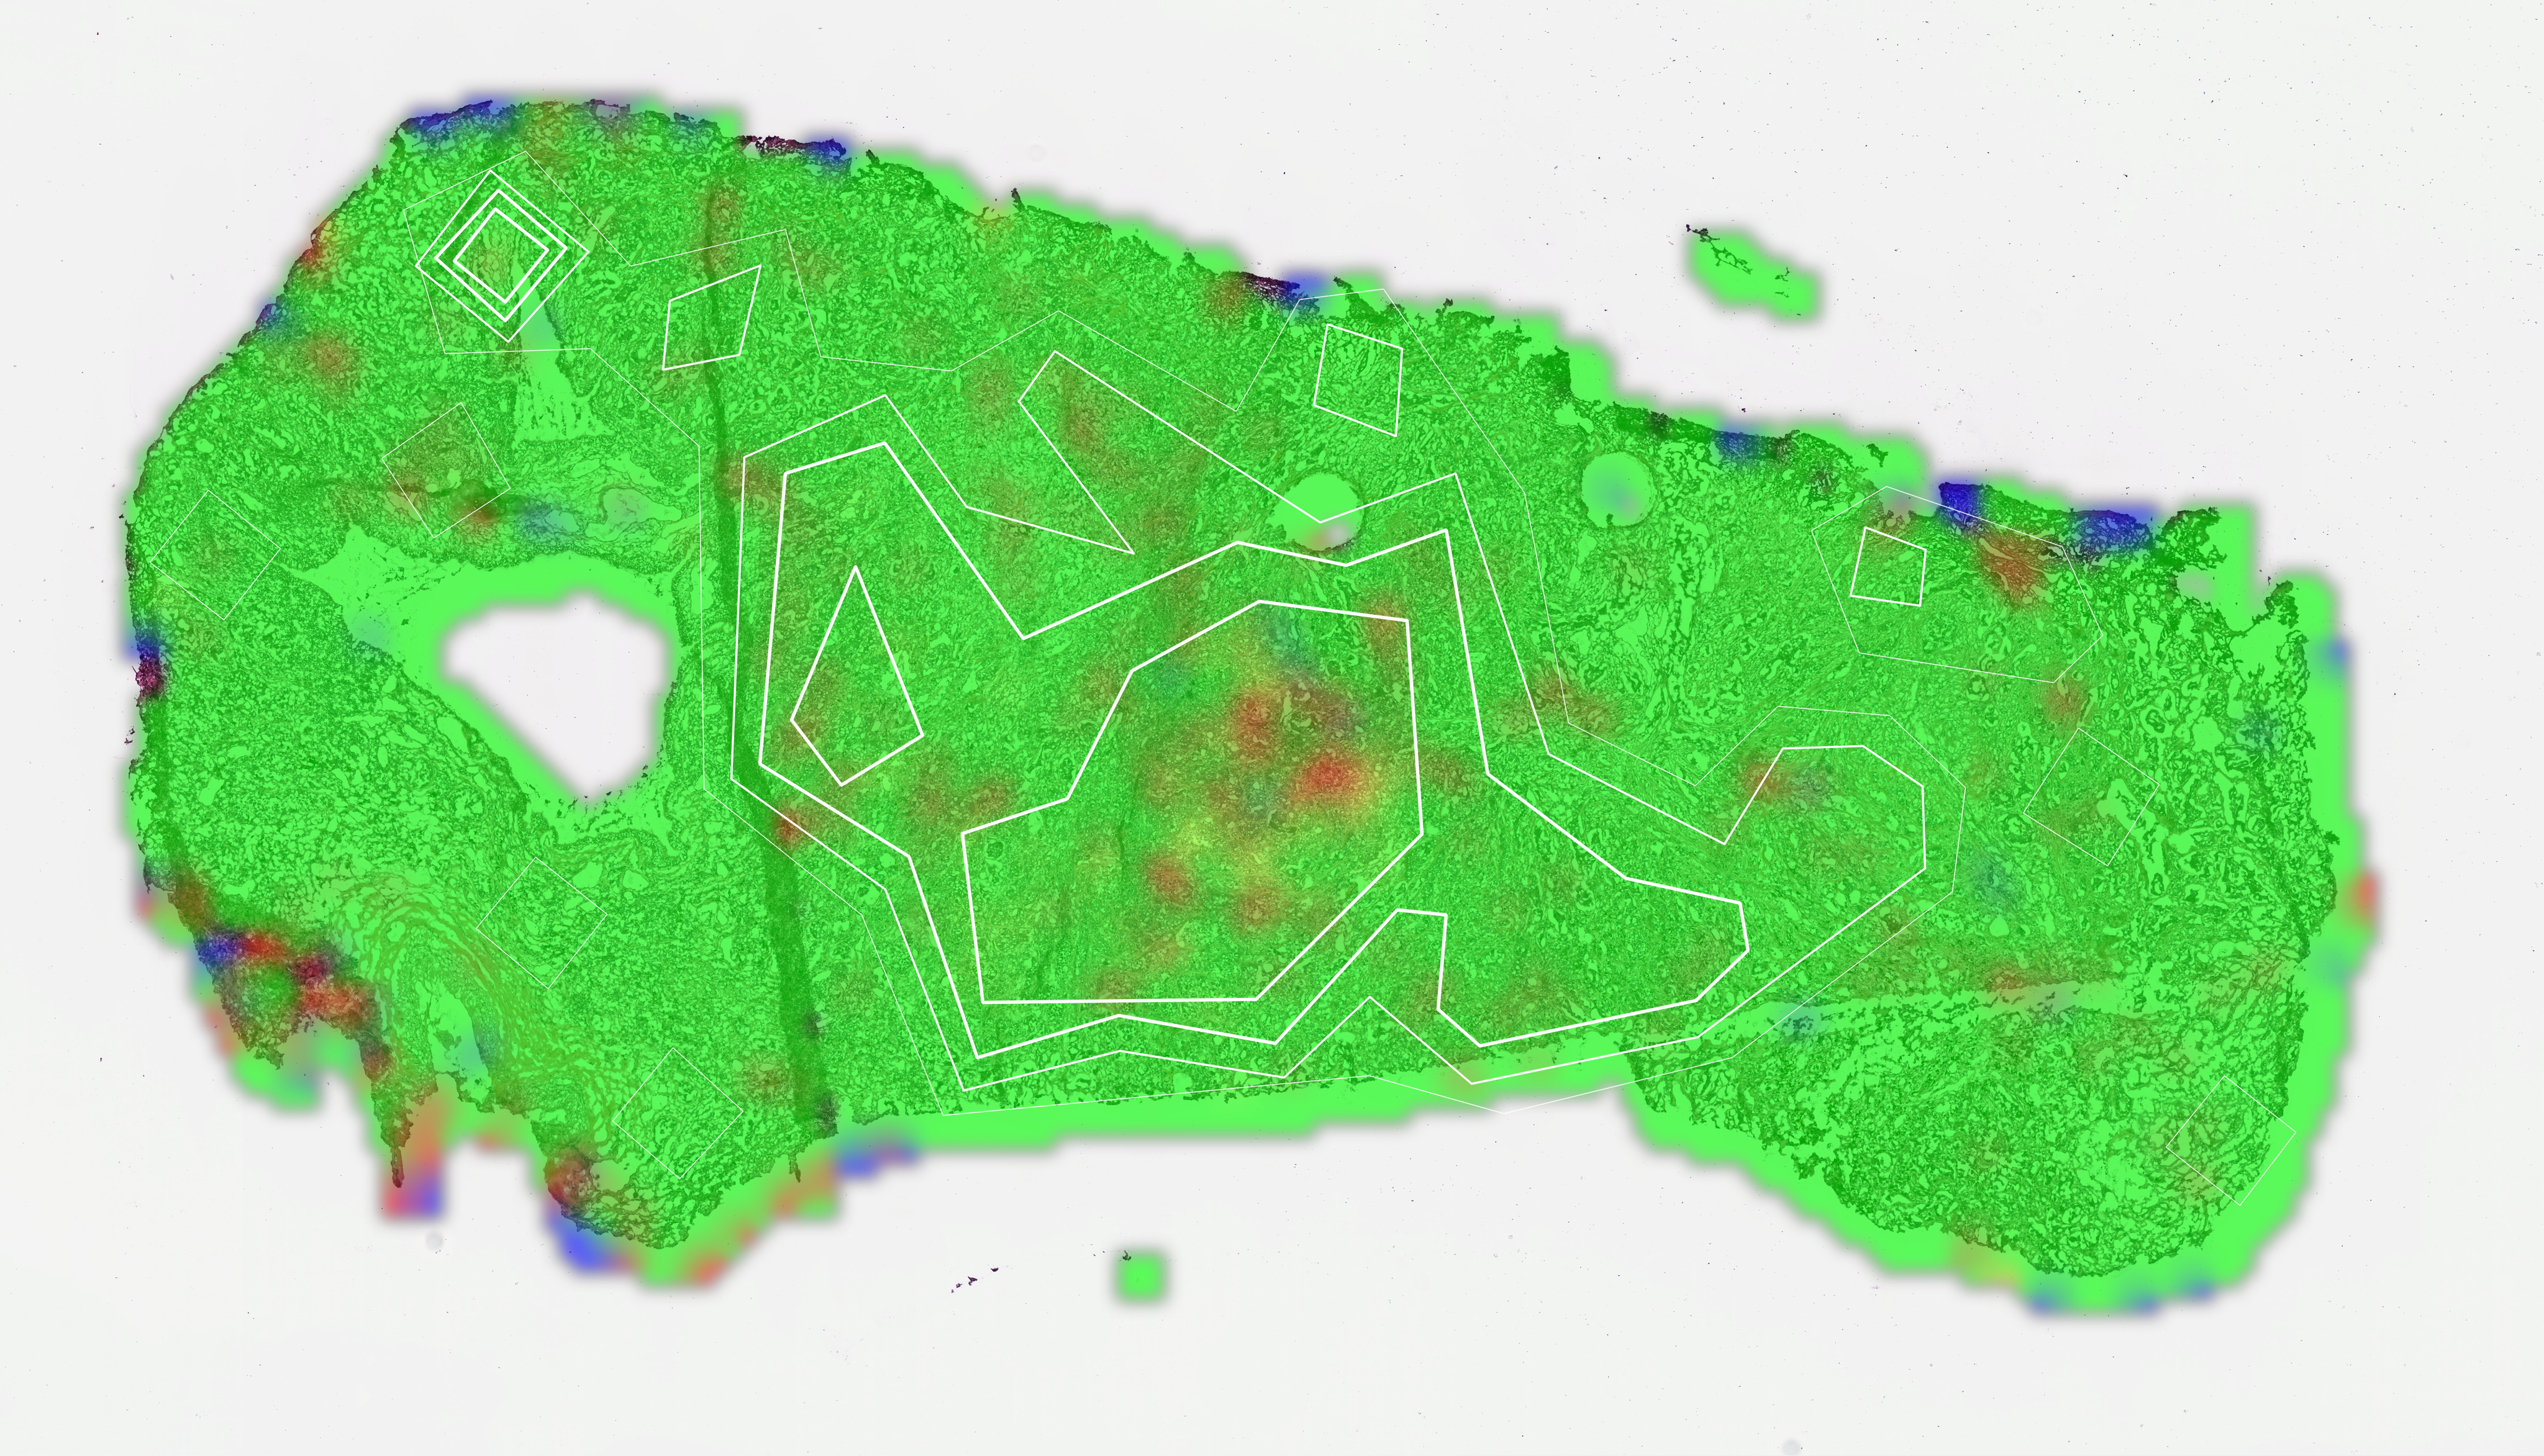
\includegraphics[width=\linewidth]{lchai_v2_TP53_TCGA-99-8025_combined}
    \caption{TP53, TCGA-99-8025 ($P=0.951$, TP).}
    \label{fig:case_tp53}
  \end{subfigure}\hfill
  \begin{subfigure}[t]{0.32\linewidth}
    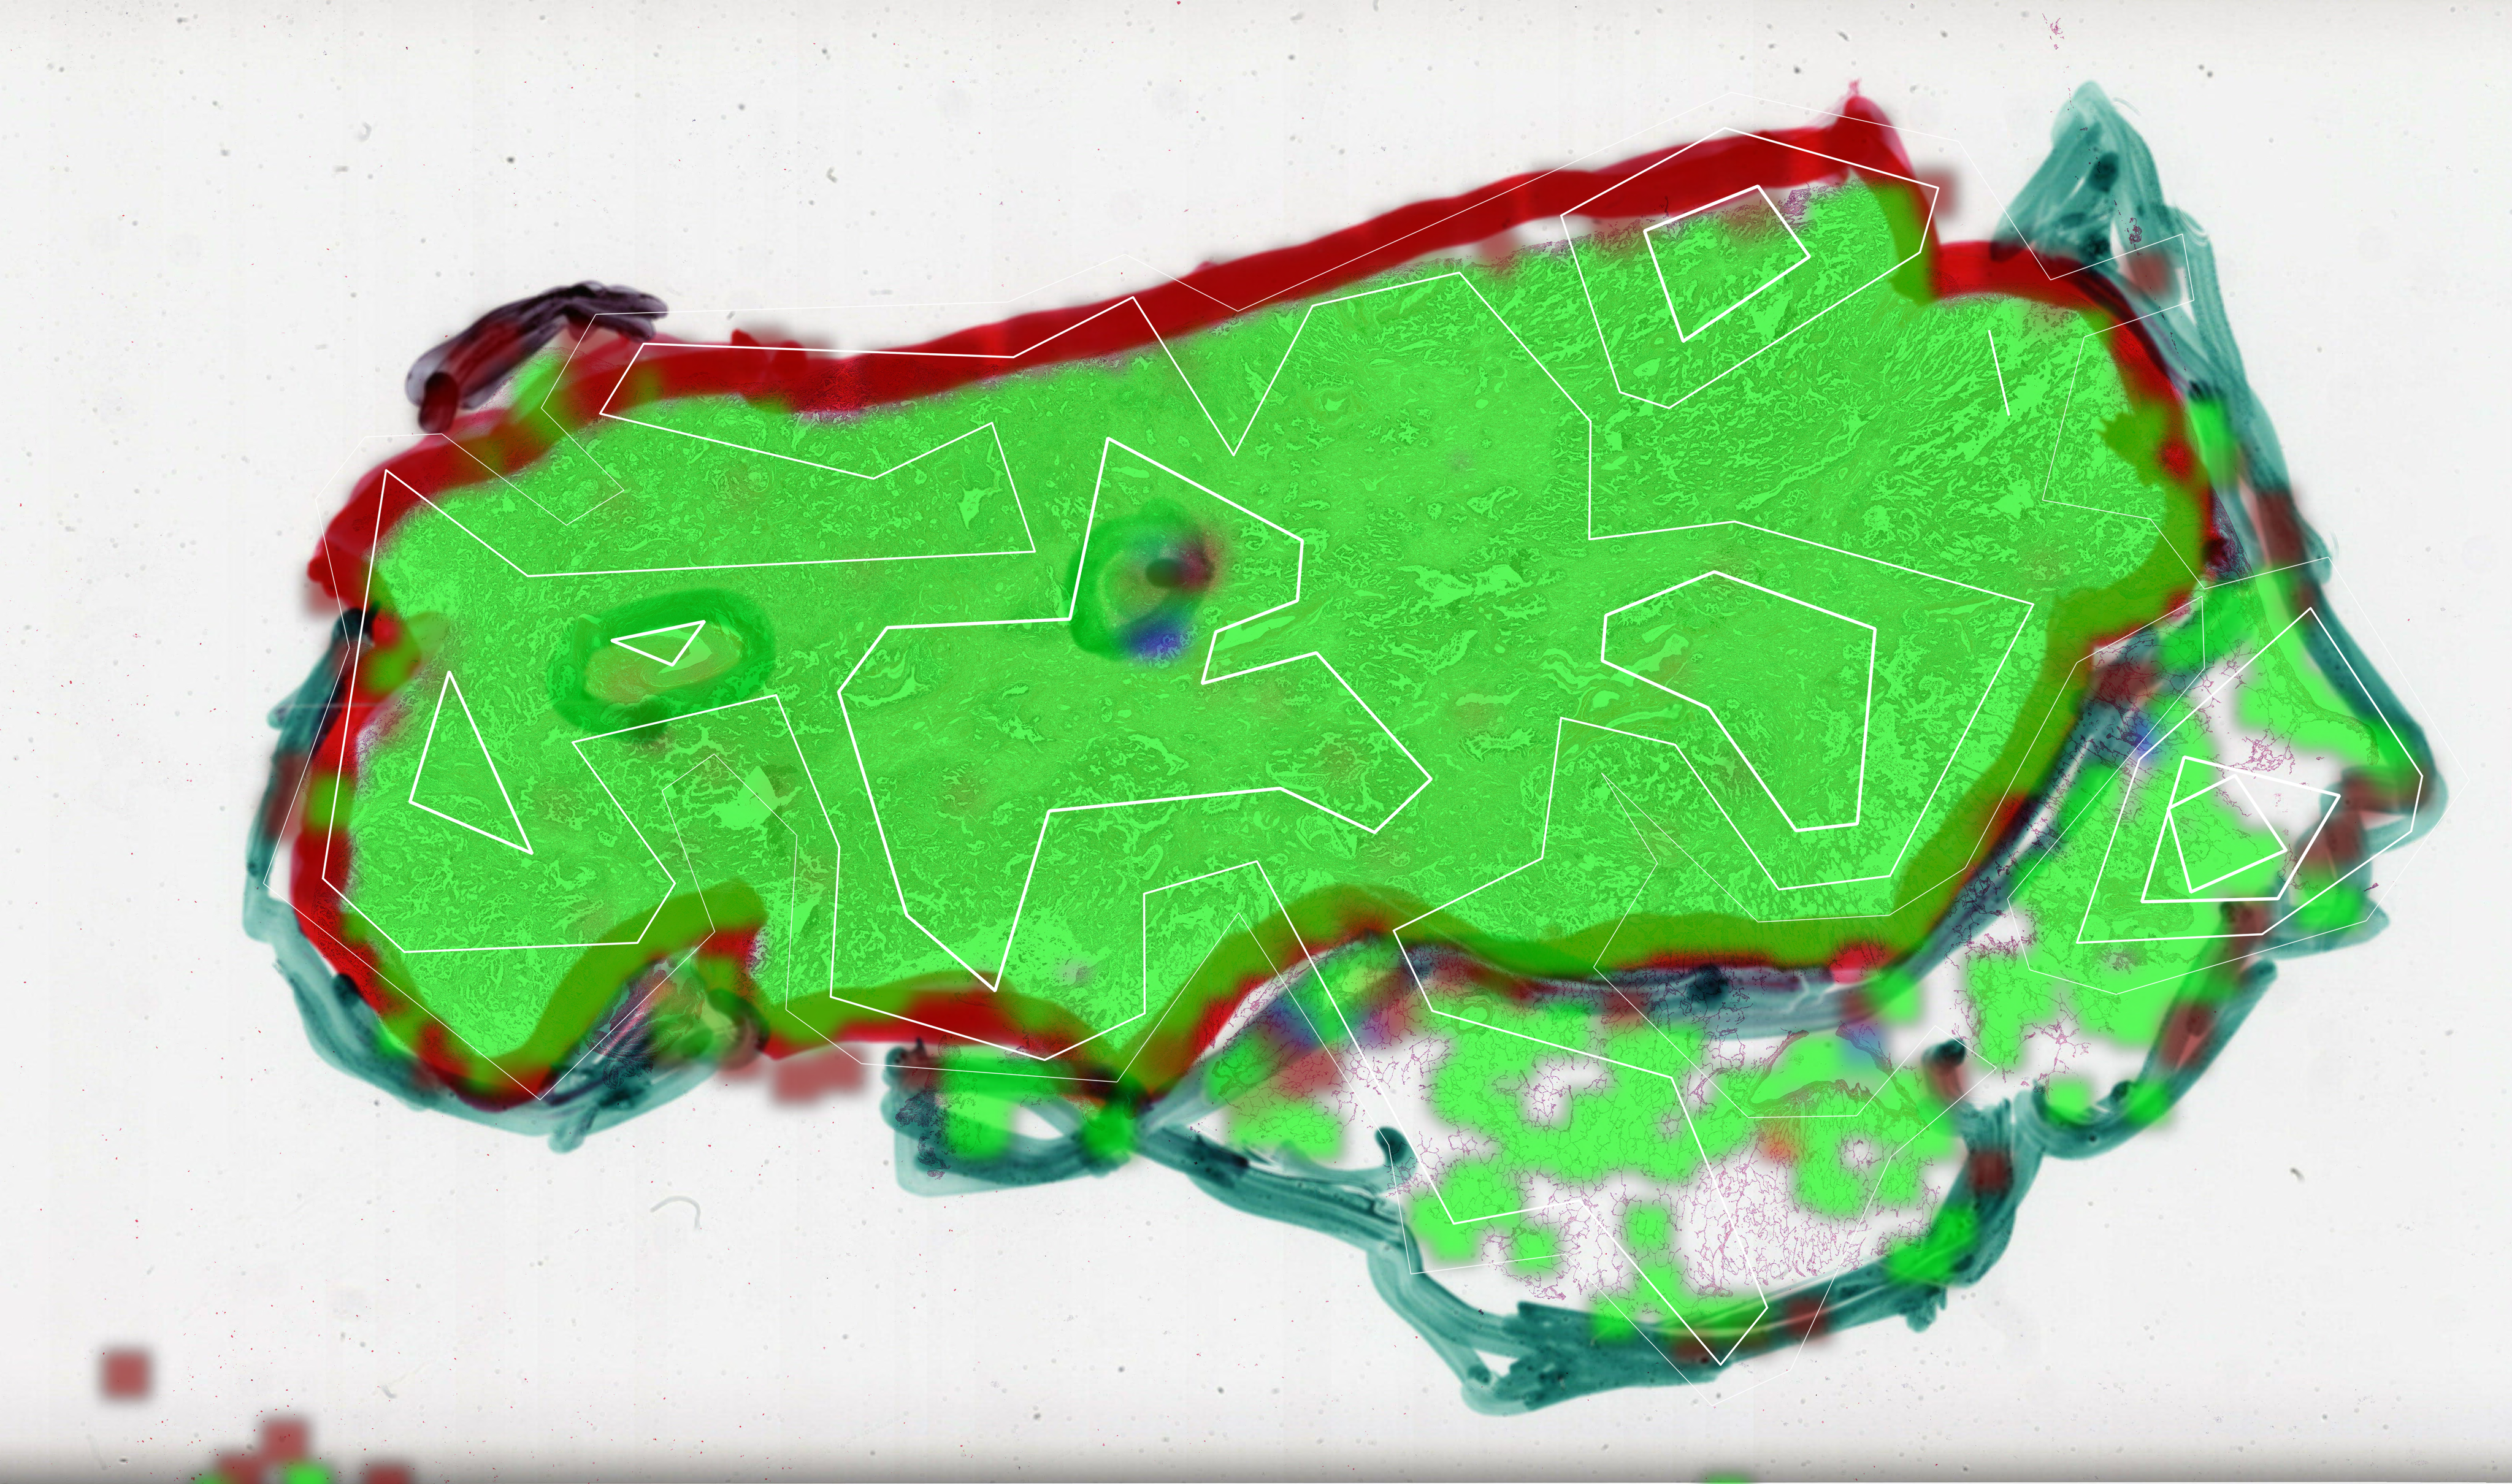
\includegraphics[width=\linewidth]{lchai_v2_EGFR_TCGA-86-8280_combined}
    \caption{EGFR, TCGA-86-8280 (TP).}
    \label{fig:case_egfr}
  \end{subfigure}\hfill
  \begin{subfigure}[t]{0.32\linewidth}
    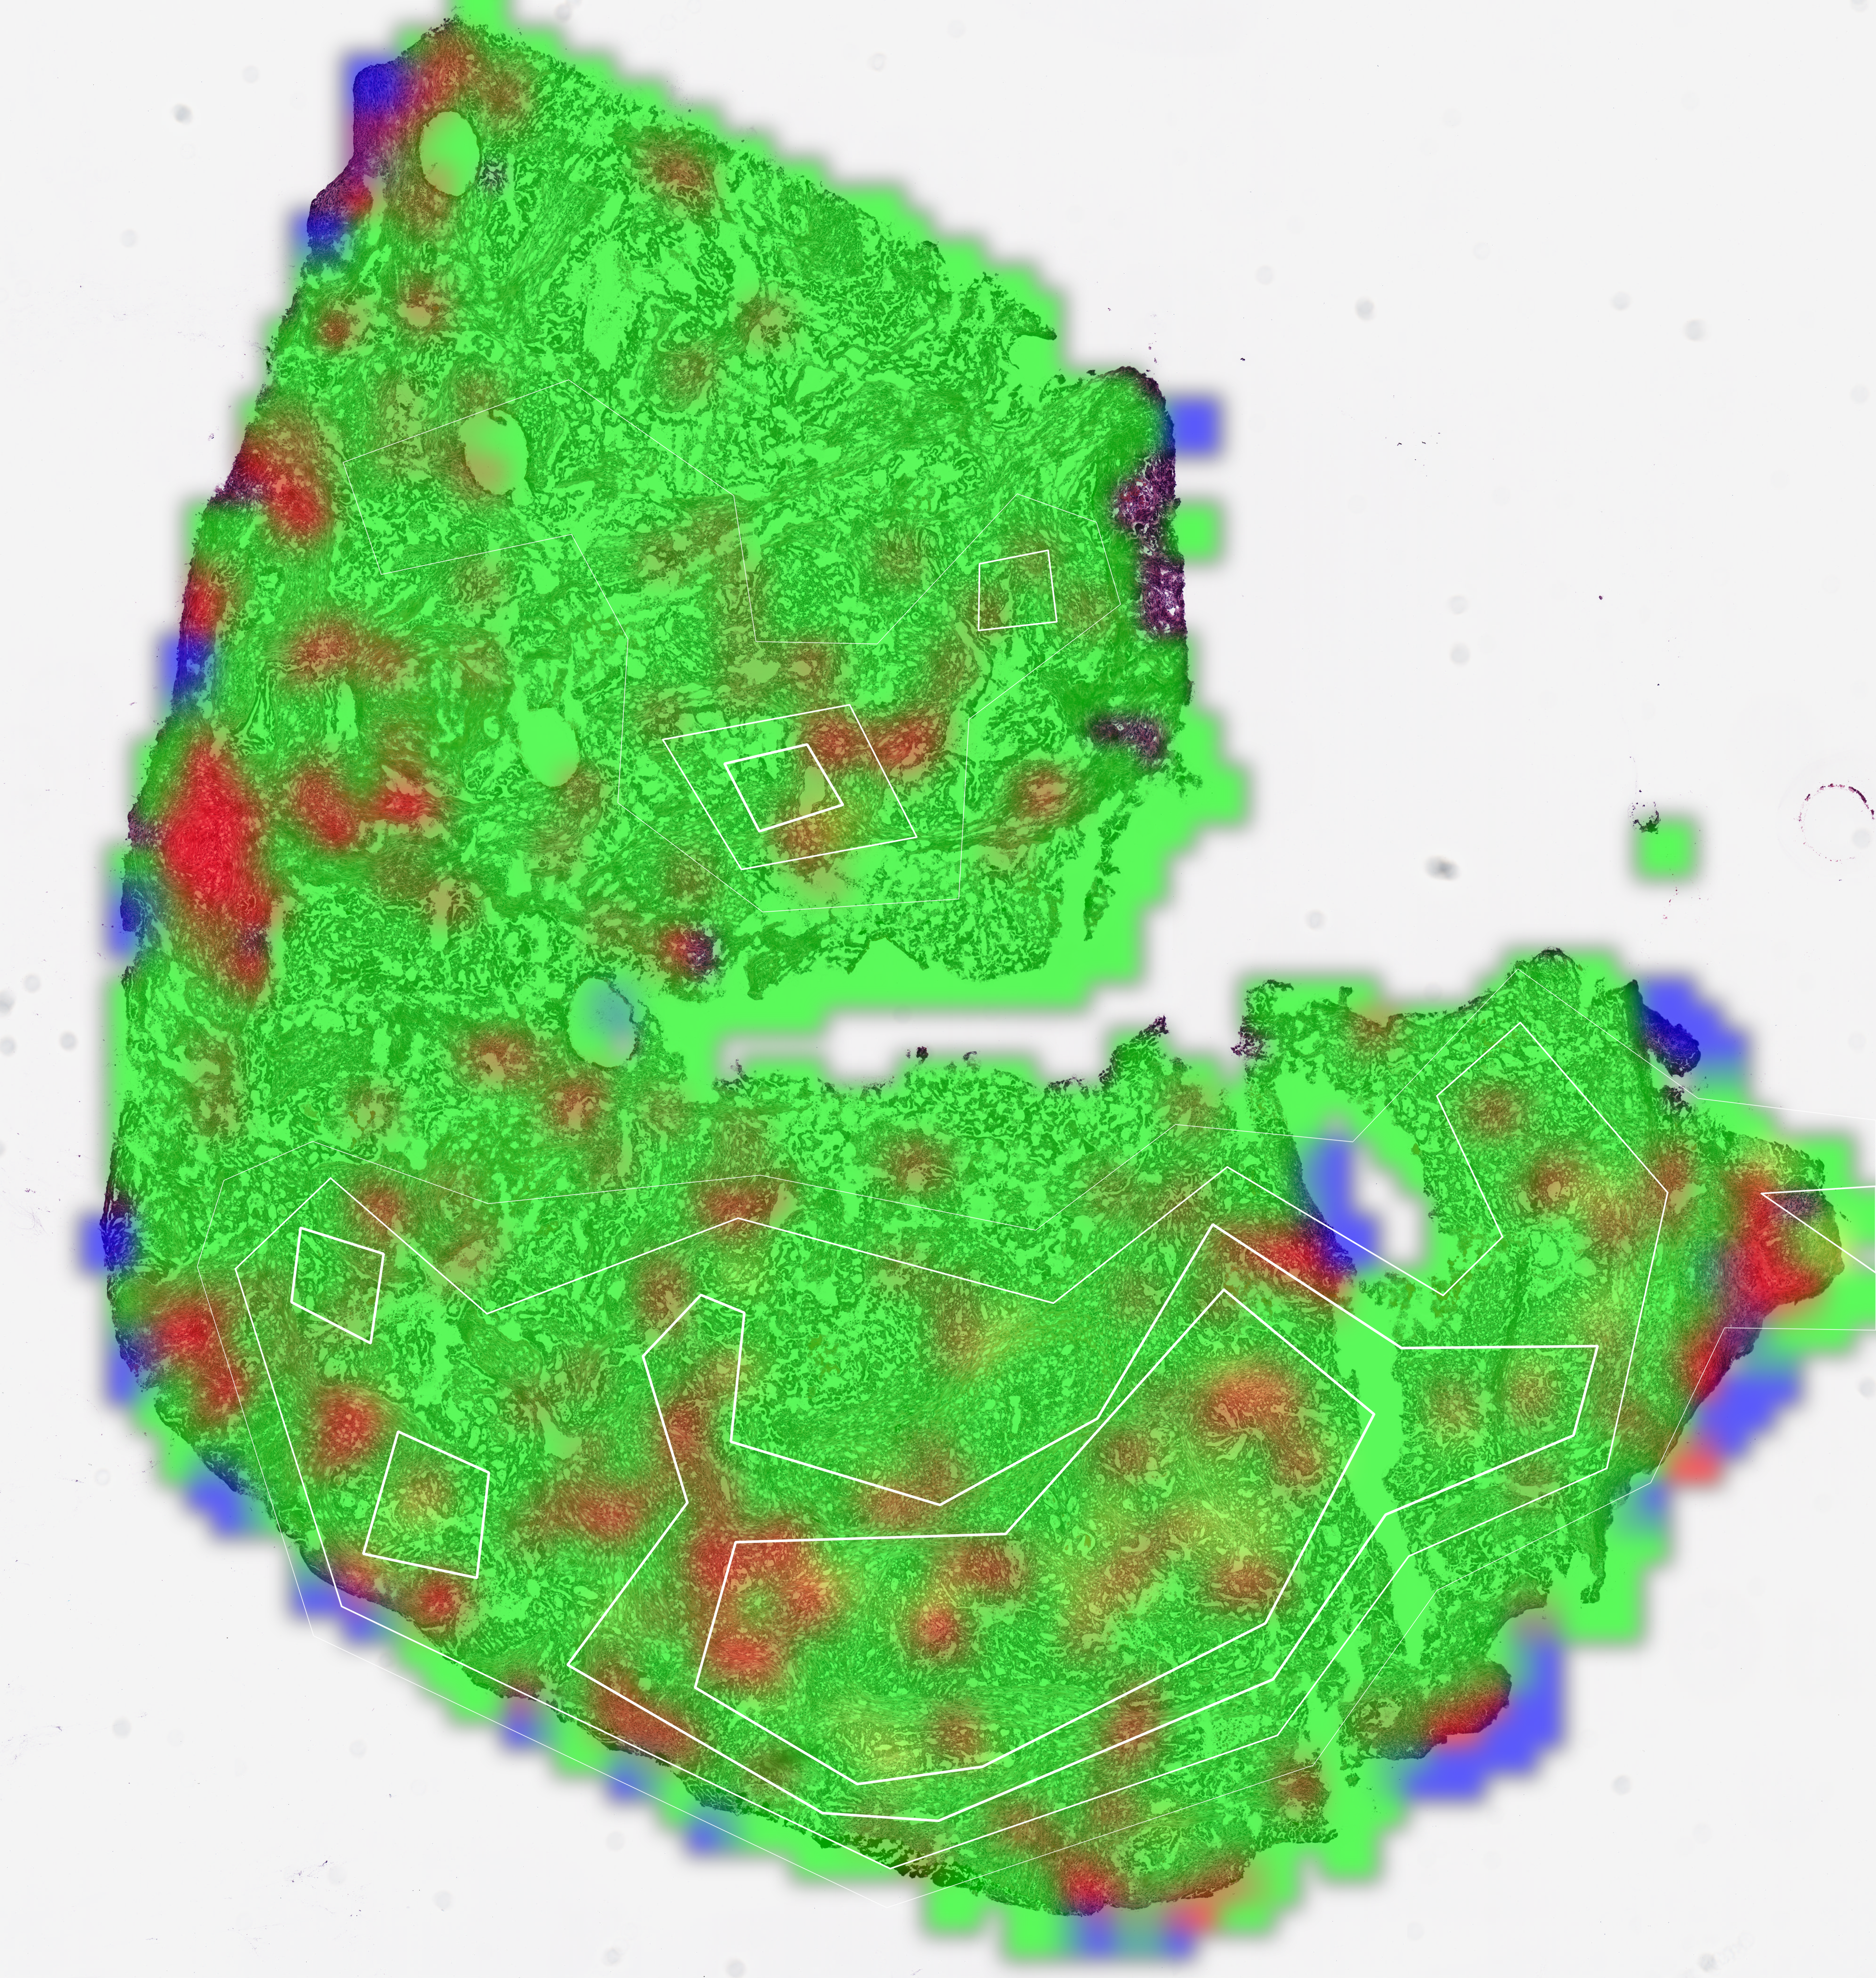
\includegraphics[width=\linewidth]{lchai_v2_KRAS_TCGA-55-7815_combined}
    \caption{KRAS, TCGA-55-7815 ($P=0.965$, IMA proxy).}
    \label{fig:case_kras}
  \end{subfigure}\\[1.2ex]
  \begin{subfigure}[t]{0.32\linewidth}
    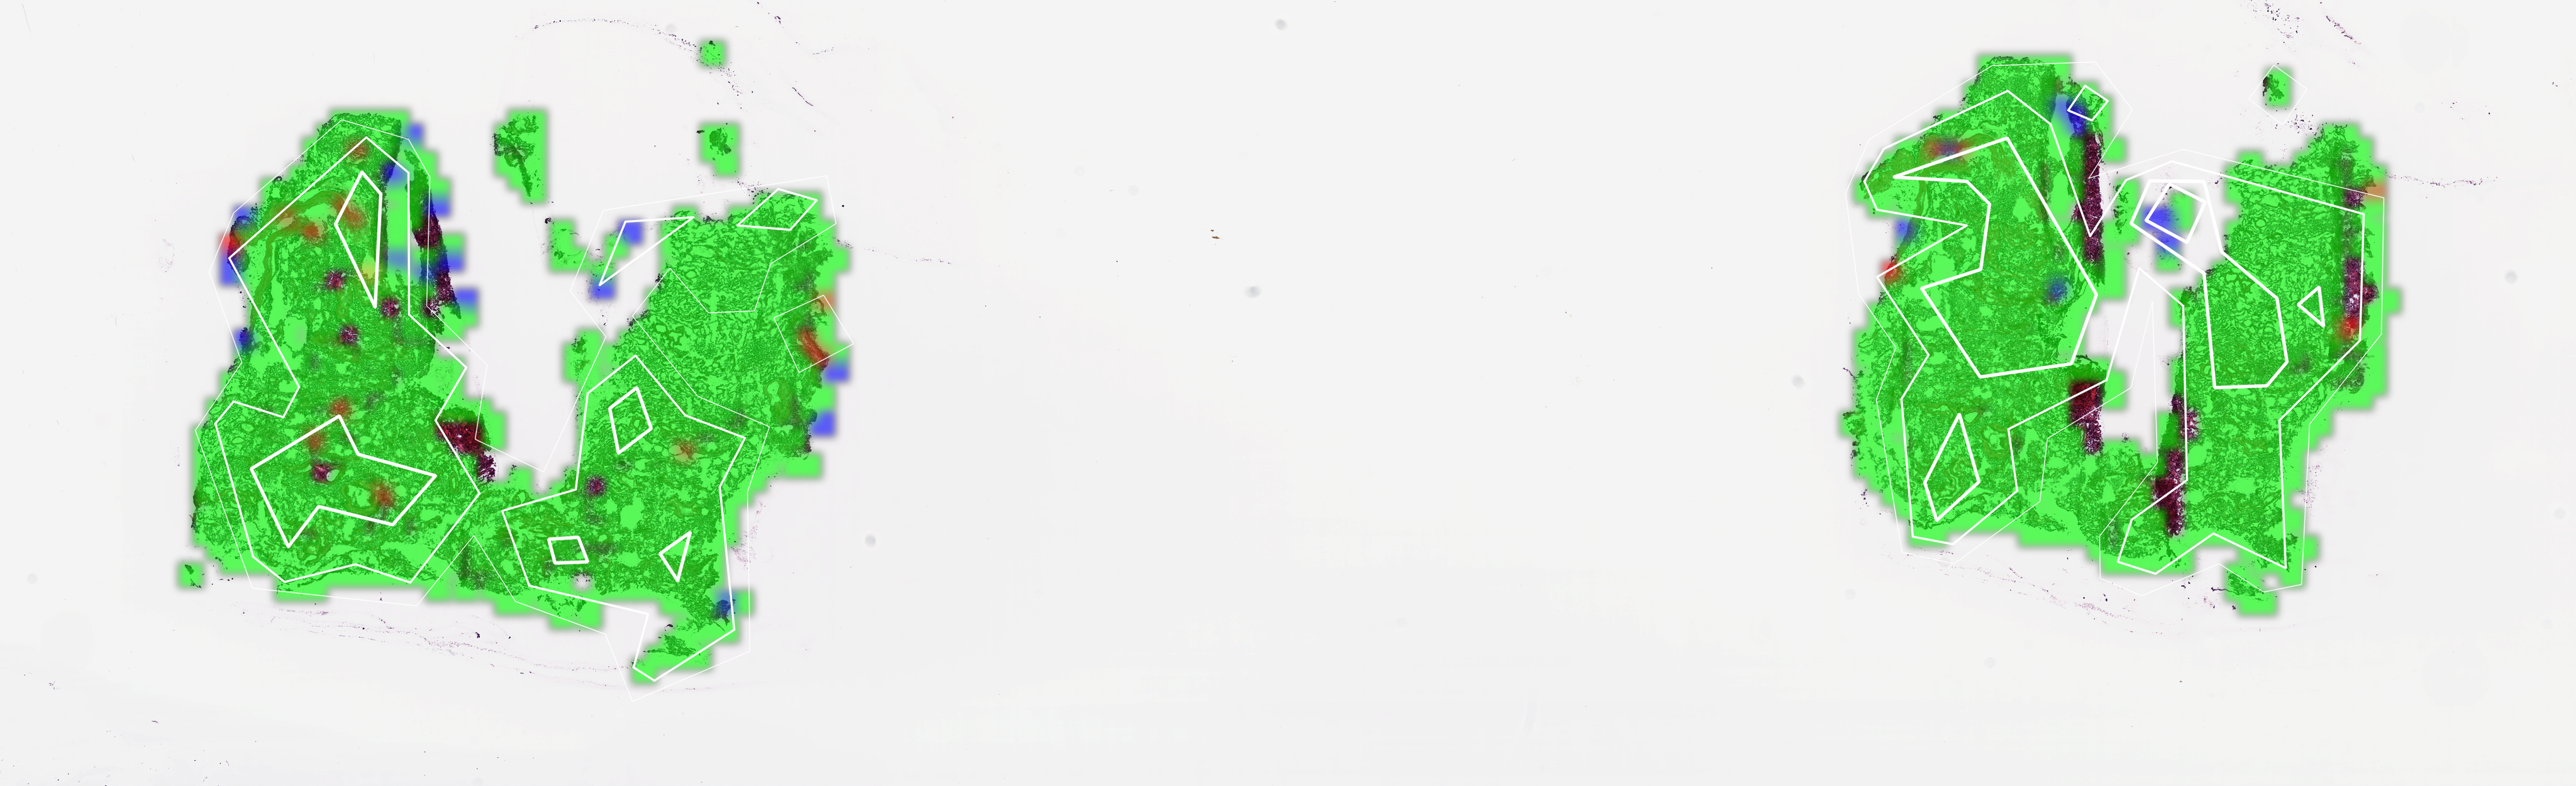
\includegraphics[width=\linewidth]{lchai_v2_STK11_TCGA-49-AAR0_combined}
    \caption{STK11, TCGA-49-AAR0 (TP).}
    \label{fig:case_stk11}
  \end{subfigure}\hfill
  \begin{subfigure}[t]{0.32\linewidth}
    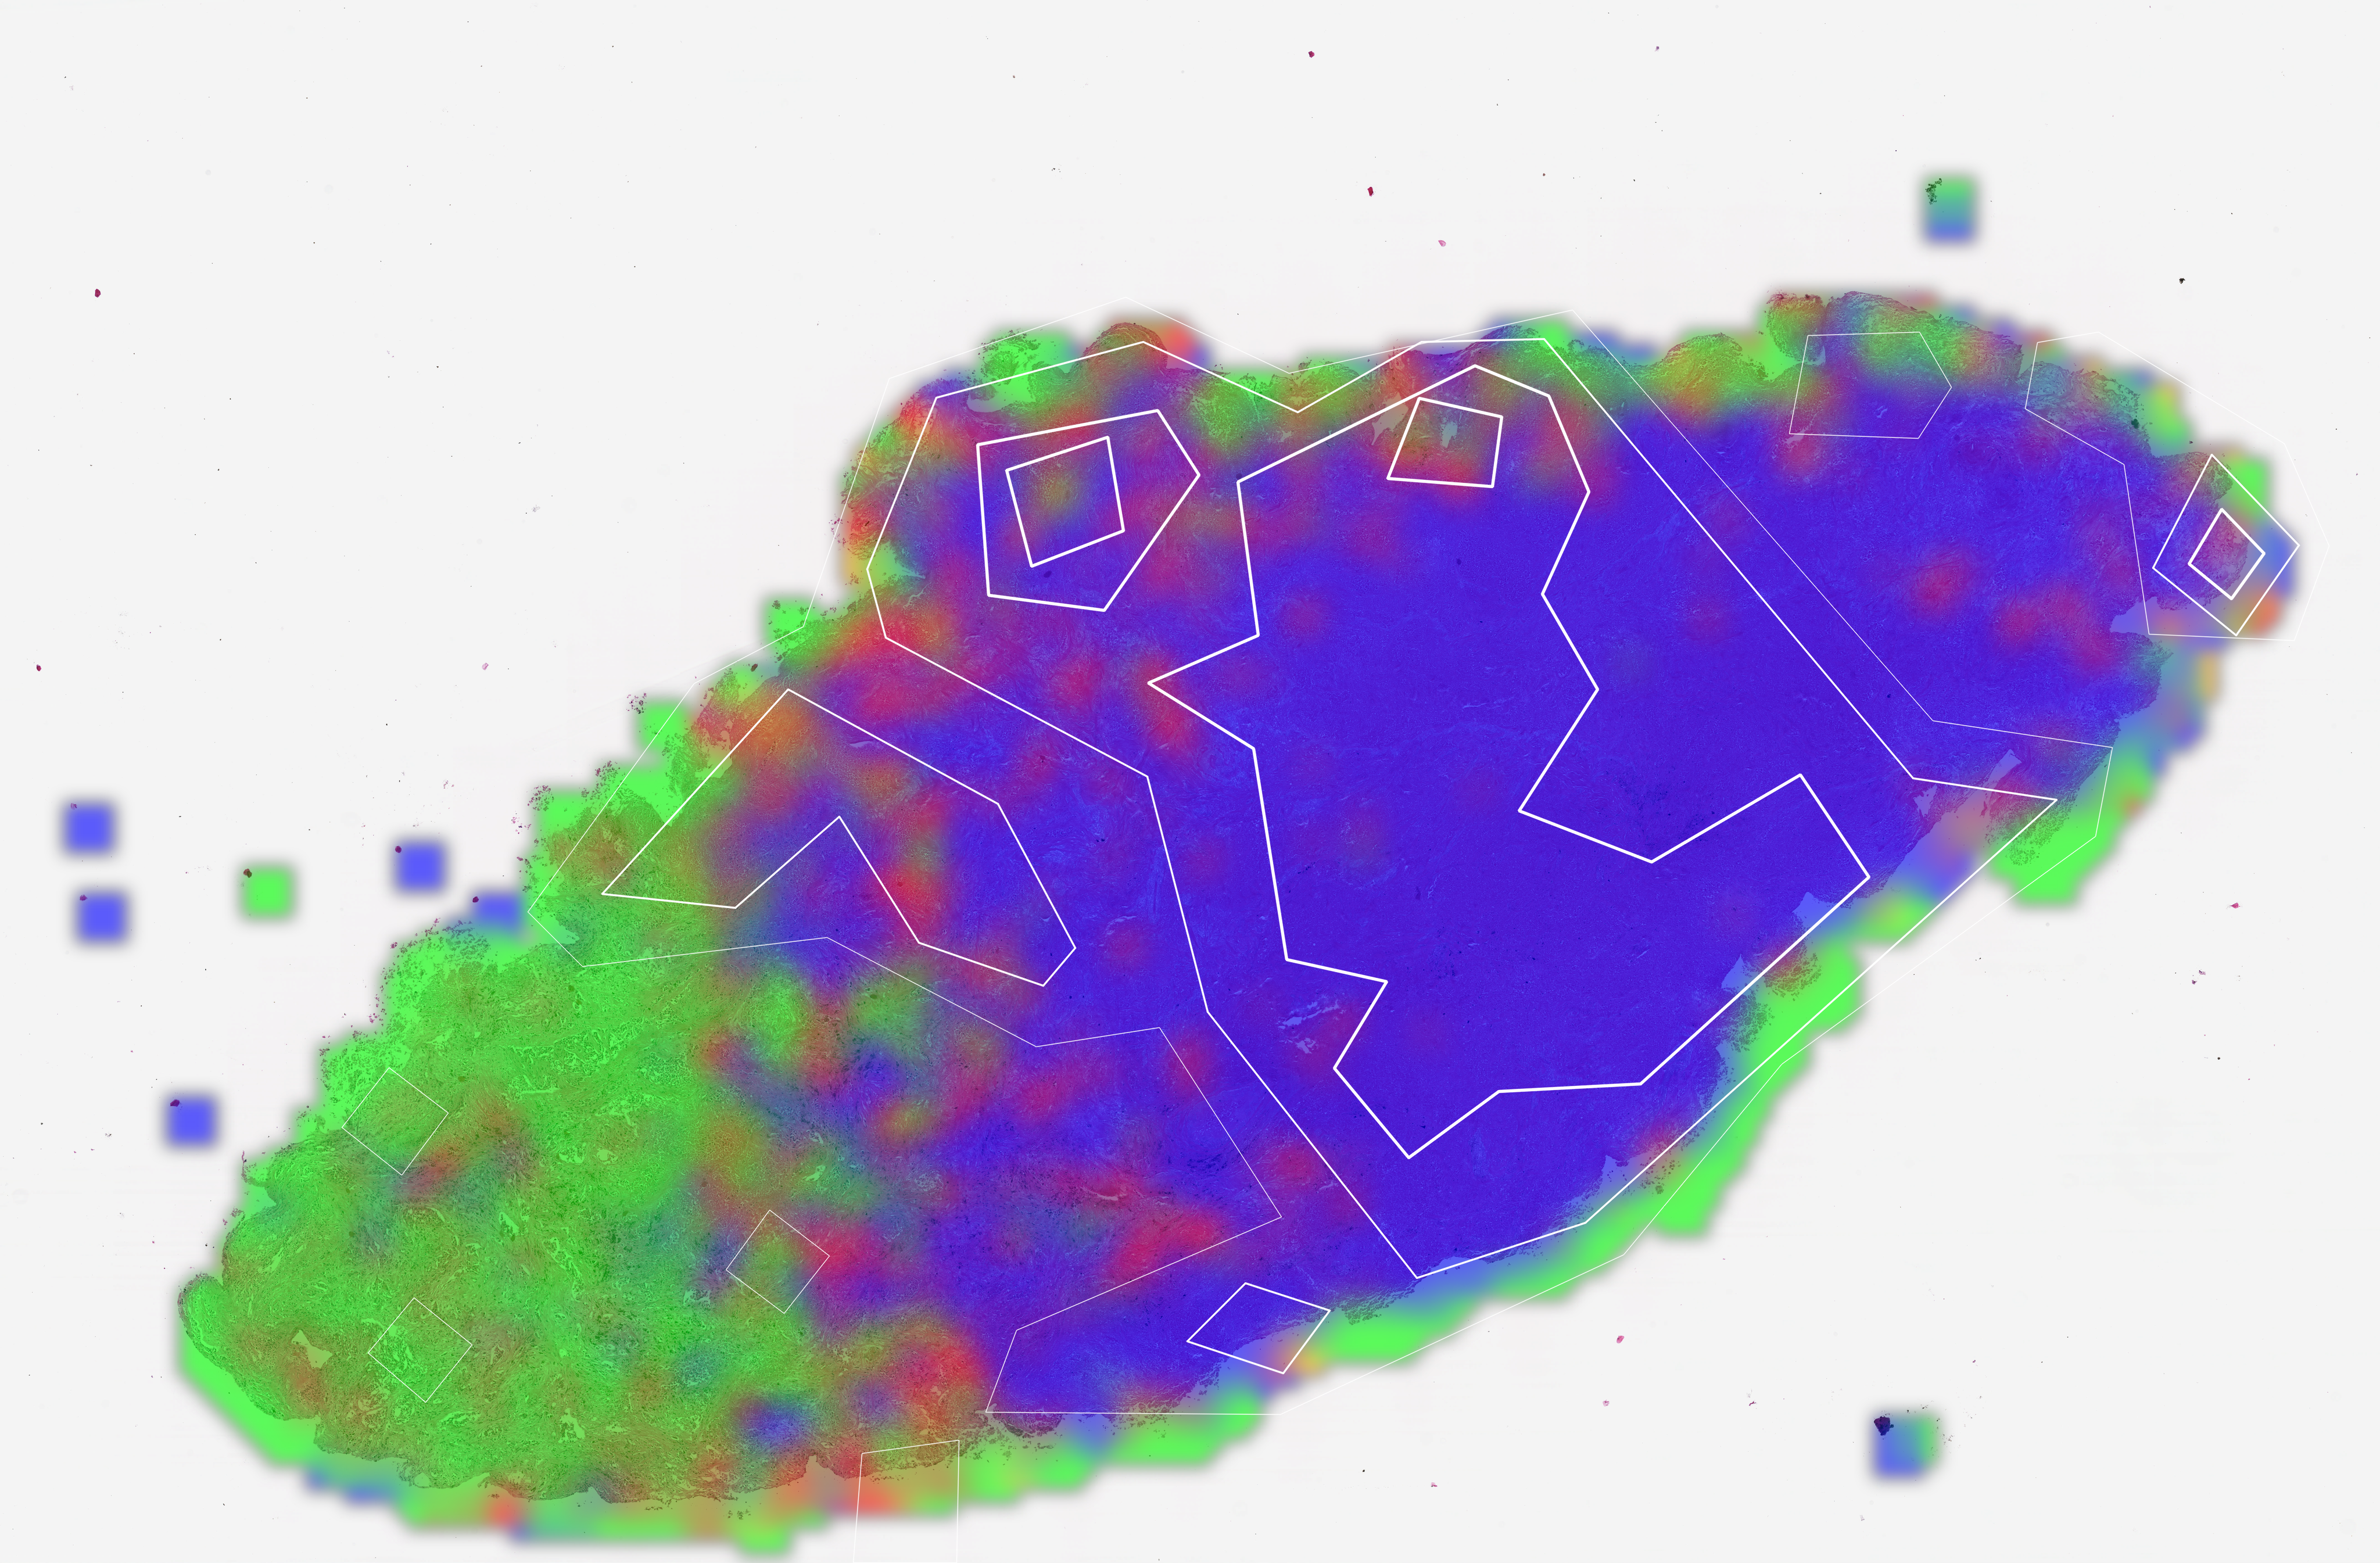
\includegraphics[width=\linewidth]{lchai_v2_KEAP1_TCGA-49-AAR9_combined}
    \caption{KEAP1, TCGA-49-AAR9 (TP).}
    \label{fig:case_keap1}
  \end{subfigure}\hfill
  \begin{subfigure}[t]{0.32\linewidth}
    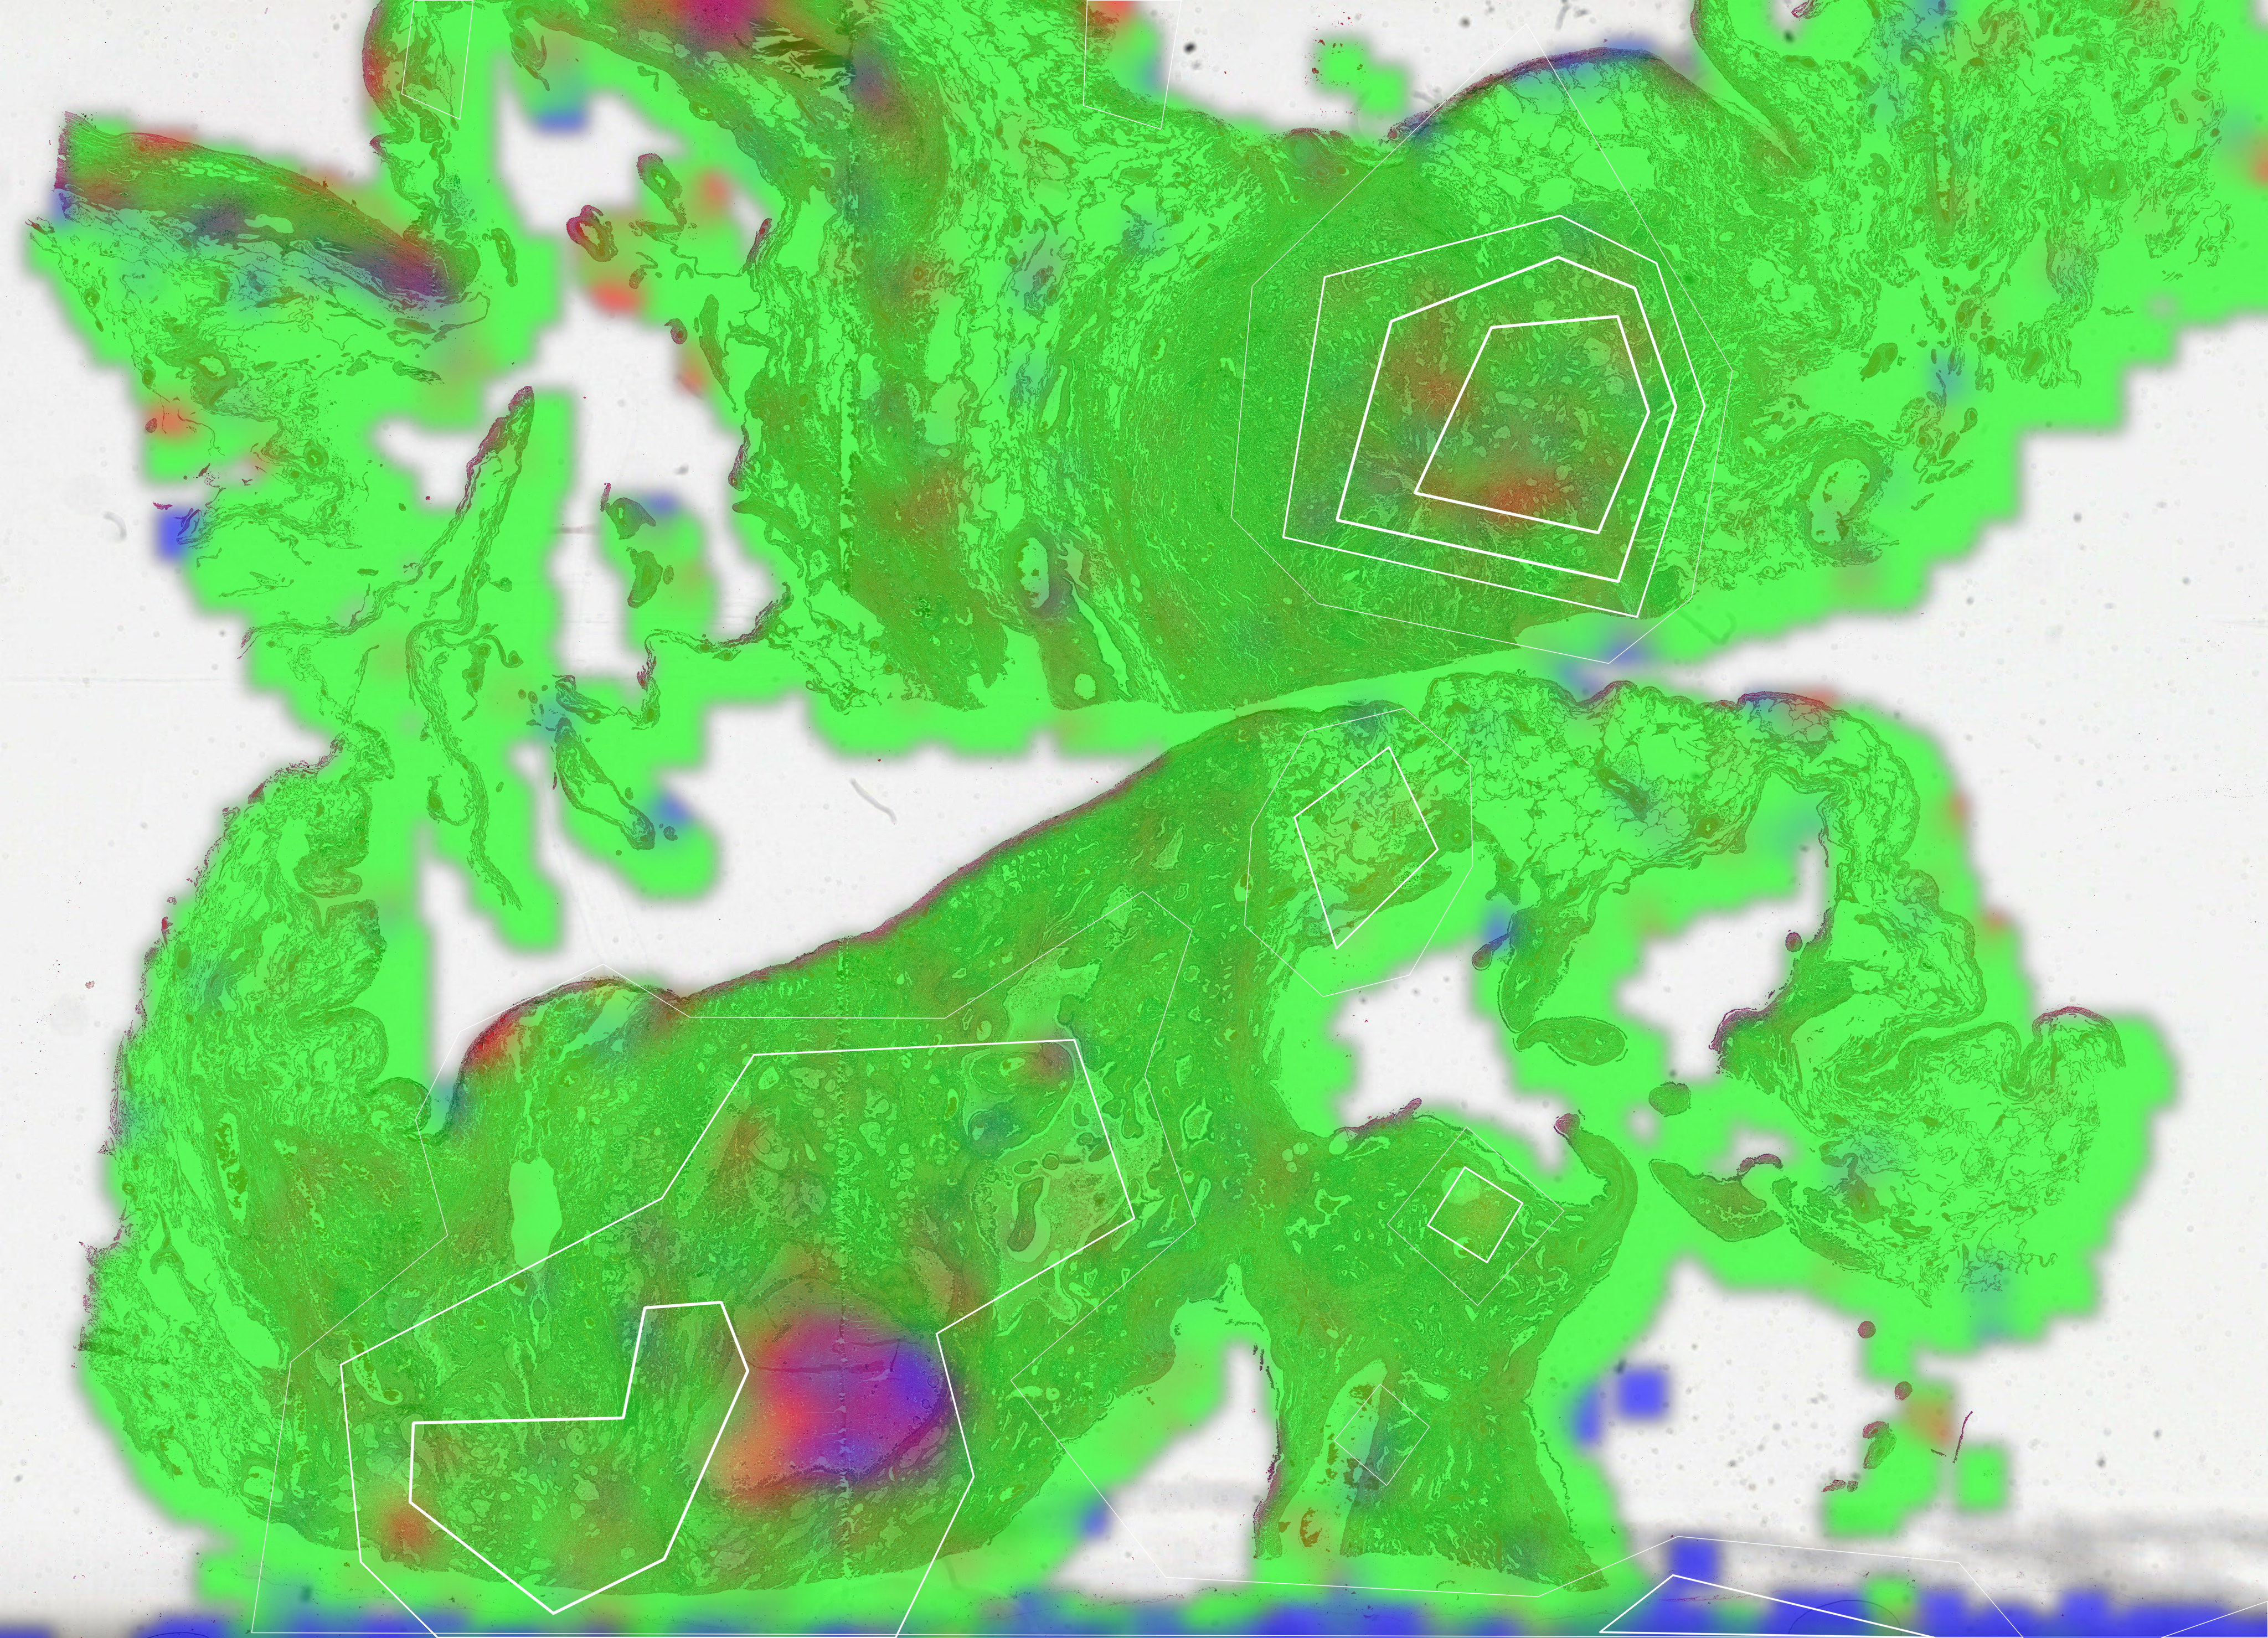
\includegraphics[width=\linewidth]{lchai_v2_RBM10_TCGA-78-7148_combined}
    \caption{RBM10, TCGA-78-7148 (TP).}
    \label{fig:case_rbm10}
  \end{subfigure}
  \caption{\textbf{Per-gene case studies.} For each of the six
  target genes, one representative true-positive slide is shown
  with the four-panel \lchai{} composite: (top-left)~\ctranspath{}
  thumbnail of the whole-slide image; (top-right)~pattern overlay
  (L2) coloured by the dominant ANORAK pattern at each tile;
  (bottom-left)~ABMIL attention map (L1) showing where the
  aggregator weighed evidence; (bottom-right)~combined L1+L2
  overlay localising the high-attention, high-pattern-saliency
  regions. The KRAS panel illustrates the value of decoupling the
  cohort-level verdict (Inconclusive at $0.609$ mean AUROC) from
  the per-slide explanation: TCGA-55-7815 is per-slide confident
  ($P=0.965$) and the L4 Choquet readout (\cref{fig:kras_proxy_b})
  localises the confidence in the lepidic$\times$solid
  co-activation. Per-slide additional examples and full SHAP
  channel decompositions appear in Extended Data.}
  \label{fig:case_grid}
\end{figure}

\cref{fig:case_grid} shows representative true-positive and
true-negative cases for each gene, juxtaposing the
\ctranspath{} thumbnail, the pattern overlay (L2), the ABMIL
attention map (L1) and the combined overlay; specifically:
TP53 \href{https://portal.gdc.cancer.gov}{TCGA-99-8025}
($P=0.951$, TP), EGFR TCGA-86-8280, KRAS TCGA-55-7815
($P=0.965$, IMA-proxy), STK11 TCGA-49-AAR0, KEAP1 TCGA-49-AAR9,
RBM10 TCGA-78-7148.
The case studies illustrate the value of decoupling the
cohort-level verdict from the per-slide explanation:
KRAS TCGA-55-7815 is per-slide confident and the L4 Choquet
readout localises the confidence in the
lepidic$\,\times\,$solid co-activation, even though the cohort
verdict for KRAS is Inconclusive.

% =====================================================================
\subsection*{Comparison with published mutation-prediction work}
% =====================================================================

\begin{table}[h!]
\centering
% Table tab:literature_comparison_resultssec — comparison of mutation prediction
% methods in NSCLC. Synced with thesis Table 2.5 (ch02_background.tex, lines
% 1299-1331): seven prior studies + this work's two MIL conditions.
% AUROC values are means or ranges across the cited paper's CV protocol;
% daggers (^\dagger) indicate values approximated from published figures.
% Wide table: wrapped in \resizebox so it scales to the printed column width.
\resizebox{\linewidth}{!}{%
\setlength{\tabcolsep}{4pt}
\begin{tabular}{l c l r l c c c c c c}
\toprule
\textbf{Study} & \textbf{Year} & \textbf{Journal} & $\boldsymbol{N}$ &
  \textbf{Method} &
  \textit{TP53} & \textit{EGFR} & \textit{KRAS} &
  \textit{STK11} & \textit{KEAP1} & \textit{RBM10} \\
\midrule
Coudray~et~al.\cite{coudray2018classification} &
  2018 & Nat.\ Med.\ & 382 & Inception-v3 e2e &
  0.733--0.86\textsuperscript{*} & 0.826 & 0.733 & 0.733\textsuperscript{*} & --- & --- \\
Kather~et~al.\cite{kather2020pancancer} &
  2020 & Nat.\ Cancer & 17{,}355 & ShuffleNet+att.\ &
  0.65--0.72$^{\dagger}$ & 0.63--0.68$^{\dagger}$ & 0.60--0.65$^{\dagger}$ & --- & --- & --- \\
Saldanha~et~al.\cite{saldanha2023npj} &
  2023 & npj Prec.\ Onc.\ & 676 & RetCCL+attMIL &
  0.65$^{\dagger}$ & 0.67$^{\dagger}$ & 0.61$^{\dagger}$ &
  0.63$^{\dagger}$ & 0.58$^{\dagger}$ & --- \\
Zhao~et~al.\cite{zhao2025deepgem} (DeepGEM) &
  2025 & Lancet Onc.\ & 3{,}637 & co-supervised MIL &
  0.82--0.96 & 0.82--0.96 & 0.82--0.96 & 0.82--0.96 & --- & --- \\
Campanella~et~al.\cite{campanella2025eagle} (EAGLE) &
  2025 & Nat.\ Med.\ & 8{,}461 & FM fine-tuning &
  --- & \textbf{0.890} & --- & --- & --- & --- \\
Wang~et~al.\cite{wang2024chief} (CHIEF) &
  2024 & Nature & 60{,}530 & FM, pan-cancer &
  $>$\,0.70 & $>$\,0.70 & --- & --- & --- & --- \\
\midrule
\multirow{2}{*}{\textbf{This work}} & \multirow{2}{*}{2026} & \multirow{2}{*}{---} & \multirow{2}{*}{\textbf{687}}
  & \piabmil{} & \textbf{0.717} & \textbf{0.694} & 0.590 & \textbf{0.695} & \textbf{0.610} & 0.640 \\
  & & & & \fcmil{} & 0.716 & 0.684 & \textbf{0.609} & 0.658 & 0.589 & \textbf{0.661} \\
\bottomrule
\end{tabular}%
}
\begin{flushleft}\footnotesize
\textsuperscript{*}Range across six genes.
$^{\dagger}$Approximate values transcribed from published figures or
supplementary bar charts.
Cohort sizes ($N$) are slide counts; CHIEF and EAGLE use proprietary
cohorts an order of magnitude larger than the public TCGA-LUAD subset
evaluated here.
This work reports six driver genes per slide simultaneously, with two
parallel MIL aggregators (\piabmil{} concatenative attention,
\fcmil{} 2-additive Choquet); prior work typically reports two to three
genes.
``---'' indicates the gene was not reported in the corresponding study;
most published studies do not report STK11, KEAP1, or RBM10 individually.
\end{flushleft}

\caption{Per-gene AUROC versus the published mutation-prediction
competition on LUAD.
This work reports six driver genes simultaneously on the public
TCGA-LUAD cohort under a single MIL aggregator;
prior work typically reports two to three driver genes on either
the same public cohort (Coudray, Saldanha, Zhao) or on proprietary
cohorts an order of magnitude larger (CHIEF, EAGLE).}
\label{tab:literature_comparison_resultssec}
\end{table}

\cref{tab:literature_comparison_resultssec} places our results
beside the published competition.
On TP53 our $0.717$ is comparable to Saldanha's $0.65$ but below
Coudray's $0.733$.
On EGFR our $0.694$ is below Coudray's $0.826$ and Campanella's
EAGLE $0.890$, both of which use proprietary cohorts an
order of magnitude larger and architectures tuned end-to-end for
EGFR specifically.
On STK11 ($0.695$), KEAP1 ($0.610$) and RBM10 ($0.661$) our
upper-tier conditions deliver per-gene numbers that are
\emph{not} reported in most prior work; STK11 and KEAP1 are
typically dropped from method papers because of their small
positive sets, and RBM10 is to our knowledge first reported
here at the per-slide level.

The cohort gap to CHIEF ($n=60{,}530$) and EAGLE ($n=8{,}461$)
is two orders of magnitude.
The contribution of this paper is not to close that gap, but to
publish \emph{what the public TCGA-LUAD cohort actually
supports} for each gene---with a Conclusive/Inconclusive
verdict, a regime-typed explanation of \emph{why}, and a
six-level interpretability stack that a pathologist can argue
against.
